%\textit{\textbf{The following section formatting is \textbf{optional}, you can also define sections as you deem fit.
%\\
%Focus on what future researchers or practitioners would find useful for reproducing or building upon the paper you choose.\\
%For more information of our previous challenges, refer to the editorials \cite{Sinha:2022,Sinha:2021,Sinha:2020,Pineau:2019}.
%}}
\section{Introduction}
% A few sentences placing the work in high-level context. Limit it to a few paragraphs at most; your report is on reproducing a piece of work, you don’t have to motivate that work.

As computational capabilities increase, deep learning models for computer vision (CV) are growing to the point where access to labeled data becomes the performance bottleneck. The introduction of BERT in 2018 enabled effective and scalable \textit{self-supervised} pre-training in Natural Language Processing (NLP) through \textit{masked autoencoding} with transformers \cite{bert}. Adapting the masked autoencoding scheme to the image domain posed two main problems: 1) architectural differences between convolutional neural networks and transformers, and 2) much lower information density in images than in written language. Dosovitskiy et al. addressed the former in 2020 with the introduction of the Vision Transformer (ViT) \cite{vit}. The difference in information density would remain a challenge until He et al. proposed the Masked Autoencoder (MAE) in 2022 \cite{mae}. By masking out a large part of the input and only encoding the visible parts, the MAE managed to perform efficient and effective self-supervised pre-training with images while keeping its design exceptionally simple \cite{mae}.
\\\\
The MAE uses pixel-wise mean squared error (MSE) as the loss function during pre-training \cite{mae}. However, it has been shown that loss functions that promote accurate reconstructions do not necessarily lead to useful representations when transferring to downstream tasks, suggesting that pixel-wise reconstruction error might be a flawed metric for measuring the quality of latent representations \cite{perceptualautoencoder, ganautoencoder}. Perceptual loss has been proposed as an alternative to pixel reconstruction loss for autoencoders and has shown improved performance in downstream tasks such as image classification and object localization \cite{perceptualautoencoder}.
\\\\
In this paper, we attempt a reproduction of \cite{mae} under significant computational constraints. We also present the Semantic Masked Autoencoder (SMAE), a novel and simple extension of the MAE which uses perceptual loss to improve the autoencoder embeddings. The datasets and backbone we rely on are significantly smaller than those used by \cite{mae}. Our main experiments are performed on Tiny ImageNet (TIN) \cite{tin} and transfer learning is performed on a low-resolution version of CUB-200-2011 \cite{cub}. As backbone, we use a ViT-Lite \cite{hassani} with 3.72M parameters, thus being two orders of magnitude smaller than ViT-Large (307M parameters) which was used as baseline in \cite{mae}. We also compare the MAE and SMAE to DINO, an alternative framework for self-supervised learning \cite{dino}.
\\\\
The contributions of this paper can be summarized as follows:
\begin{itemize}
    \item We reproduce the results of \cite{mae} at a much lower scale. Through ablation studies, we settle on the same masking ratio and masking strategy as in \cite{mae}. We demonstrate favorable performance with MAE compared to supervised learning and a comparable SSL method (DINO). Models pre-trained with MAE are also shown to generalize well when transferred to another dataset.
    
    \item We demonstrate that the proposed SMAE extension improves the transfer performance of the MAE on CUB, when paired with an appropriate masking strategy.
\end{itemize}

\subsection{Scope of reproducibility}
\label{sec:claims}

%Introduce the specific setting or problem addressed in this work, and list the main claims from the original paper. Think of this as writing out the main contributions of the original paper. Each claim should be relatively concise; some papers may not clearly list their claims, and one must formulate them in terms of the presented experiments. (For those familiar, these claims are roughly the scientific hypotheses evaluated in the original work.)
This paper aims to reproduce a subset of the main claims made by He et al. in the paper "Masked Autoencoders Are Scalable Vision Learners" \cite{mae}. The main claims made by He et al. are:
\begin{enumerate}
    \item \label{nontrivial} Masking out a large part of the input image uniformly at random yields a nontrivial and meaningful self‐supervisory task. 
    \item \label{generalization} Masked autoencoding allows for learning models that generalize well.
    \item \label{scalability} The MAE is a scalable and efficient method in the sense that pre-training larger models is tractable and improves performance without overfitting to training data.
\end{enumerate}
With respect to our restricted computational budget, \textbf{we set out to investigate claims \ref{nontrivial} and \ref{generalization}}. We aim to investigate claim \ref{nontrivial} by 1) ablating the masking ratio, 2) ablating the masking method, and 3) pre-training with MAE and fine-tuning on TIN. We aim to investigate claim \ref{generalization} by pre-training with MAE on TIN and transferring the encoder to image classification on CUB. By further developing the idea of masked autoencoding through the use of perceptual loss in our proposed SMAE, we aim to provide additional evidence in support of claim \ref{generalization}.

%A claim should be something that can be supported or rejected by your data. An example is, ``Finetuning pretrained BERT on dataset X will have higher accuracy than an LSTM trained with GloVe embeddings.''
%This is concise, and is something that can be supported by experiments.
%An example of a claim that is too vague, which can't be supported by experiments, is ``Contextual embedding models have shown strong performance on a number of tasks. We will run experiments evaluating two types of contextual embedding models on datasets X, Y, and Z."

%This section roughly tells a reader what to expect in the rest of the report. Clearly itemize the claims you are testing:

%Each experiment in Section~\ref{sec:results} will support (at least) one of these claims, so a reader of your report should be able to separately understand the \emph{claims} and the \emph{evidence} that supports them.

%\jdcomment{To organizers: I asked my students to connect the main claims and the experiments that supported them. For example, in this list above they could have ``Claim 1, which is supported by Experiment 1 in Figure 1.'' The benefit was that this caused the students to think about what their experiments were showing (as opposed to blindly rerunning each experiment and not considering how it fit into the overall story), but honestly it seemed hard for the students to understand what I was asking for.}

\section{Background}
\label{sec:background}
This section presents the relevant background for the SMAE, our extension of the MAE which uses perceptual similarity to improve the autoencoder embeddings. 

\subsection{Perceptual Similarity}
\label{sec:percep}
Perceptual Similarity is a way of measuring the distance between two images. Originally proposed by Zhang et al. \cite{perceptual}, this method relies on convolutional neural networks' ability to extract semantic representations of images. This leads to a metric that is more consistent with the human visual system, as it promotes closeness of high-level structures. When used as a loss function to train autoencoding models, \textit{perceptual loss} enables learning robust representations of the input images, as opposed to pixel-space loss functions that encourage color reproduction \cite{perceptualautoencoder}. Employing perceptual loss has also been observed to significantly improve the usefulness of embeddings when training autoencoders in an adversarial setting \cite{ganautoencoder}.

\subsection{Semantic Masked Image Modelling}
\label{sec:smim}
Masked Image Modelling (MIM) is a method for self-supervised learning in CV, which involves masking parts of the input images and training models on this partial information. BEiT \cite{beit} is a recent method that reconstructs discretized tokens from masked images; taking inspiration from BERT pre-training in NLP \cite{bert}. Semantic Masked Image Modelling (SMIM) brings perceptual loss to MIM. SMIM is an approach to improving the usefulness of embeddings when performing MIM, which has become a trend as of the last year. PeCo, a concurrent work to ours, is one such technique; extending the BEiT method by using perceptual similarity as loss function when learning the visual words used as MIM targets. PeCo demonstrates state-of-the-art performance on ImageNet-1K image classification \cite{peco}. BootMAE is another SMIM method. It is an extension of the MAE which uses a temporal ensemble of an MAE model as a perceptual critic during pre-training \cite{bootmae}. Compared to BootMAE, our SMAE has the advantage of being exceedingly simple in its design.

\section{Methodology}
%Explain your approach - did you use the author's code, or did you aim to re-implement the approach from the description in the paper? Summarize the resources (code, documentation, GPUs) that you used.
We re-implemented the MAE from the description provided in the paper without consulting the author's published code. We implemented the ViT model and perceptual loss from scratch. For DINO, we used the officially published code \cite{dino}. Our perceptual critic implements the SqueezeNet model from Torchvision \cite{torchvision}. The following sections outline our methodology; detailing the models, datasets, and hyperparameters as well as the experimental setup and computational resources used.  

\subsection{Masked Autoencoder}
%Include a description of each model or algorithm used. Be sure to list the type of model, the number of parameters, and other relevant info (e.g. if it's pretrained). 
\begin{figure}[H]
    \centering
    \includegraphics[width=.5\textwidth]{img/mae_fonted.pdf}
    \vspace{-1mm}
    \caption{The MAE architecture. A large portion of the input image is masked and only non-masked patches are encoded. Mask tokens are injected into the encoded sequence before decoding, resulting in a computationally efficient MIM scheme with a non-trivial reconstruction task. Figure from \cite{mae}.}
    \label{fig:mae}
\end{figure}
The MAE is an autoencoder-type framework for MIM. A large portion of the image is masked before being fed to an encoder, consisting of a ViT, which creates a latent representation of the unmasked input. The decoder, which is a lightweight ViT, reconstructs the entire image from the latent representation created by the encoder (see Figure \ref{fig:mae}). After pre-training on unlabeled data, the decoder is discarded, as the main interest lies in transferring the encoder to downstream tasks. Regarding the reconstruction target, \cite{mae} found that downstream performance was improved by: 1) only computing the loss for masked patches, and 2) patch-wise normalizing the target pixel values.

\subsection{Masking}
The MAE stands out in that it masks a large portion of the input image. He et al. argue that this rules out solving the task by simply extrapolating from nearby unmasked patches and motivates the encoder to learn meaningful representations of the input \cite{mae}. In order to validate this claim, we ablate the ratio of masked patches in our experiments.
\\\\
The findings of \cite{mae} suggest that uniform random masking of patches is the most effective masking strategy. However, \cite{bootmae} found that masking large random blocks was more effective when using perceptual loss; suggesting that reconstructing large blocks is a difficult task for pixel regression while being helpful for a perceptual model in reasoning about the semantic structure. We decided to ablate the masking strategy for all of our models, to investigate its effect on the learned representations. 

\subsection{Semantic Masked Autoencoder}
We propose the SMAE, which extends the MAE by incorporating perceptual loss \cite{perceptual}. Instead of only reconstructing pixels, the SMAE objective is to minimize a combination of pixel-wise loss $\mathcal{L}_{pixel}$ and perceptual loss $\mathcal{L}_{percep}$: 

\begin{equation}
    \mathcal{L}_{SMAE} = \left(1-\alpha\right)\mathcal{L}_{pixel} + \alpha\mathcal{L}_{percep}
\end{equation}

Using $\alpha=0$ reduces to the MAE objective and $\alpha=1$ implies using only perceptual loss. Our implementation of perceptual loss largely follows that of \cite{perceptualautoencoder}. To avoid using a critic pre-trained on larger datasets, we train a SqueezeNet v1.1 \cite{squeezenet, torchvision} from scratch on TIN and use it as a critic in the perceptual loss. The original image and the reconstruction are fed to the critic, from which the learned representations are extracted. In order to preserve spatial information, the representations are extracted at an early stage in the critic network, as was argued for in \cite{perceptualautoencoder}. Finally, the perceptual loss is computed as the MSE between the representation of the original image and the reconstruction. Formally, let $f$ denote the MAE and $g$ denote the SqueezeNet v1.1 up until and including the second \textit{Fire} module. The perceptual loss between a sample $x$ and its reconstruction $f(x)$ can then be formulated as:

\begin{equation}
    \mathcal{L}_{percep} = \frac{c}{d}\sum_i^d \left(g(x) - g(f(x))\right)^2
\end{equation}

where $d$ is the dimensionality of the extracted representations and $c$ is a scaling factor used to ensure $\mathcal{L}_{percep}$ and $\mathcal{L}_{pixel}$ are of similar scale. In practice, we set $c$ before optimization, to the ratio between the initial pixel-wise and perceptual loss values. We tried using an uncertainty-based weighting of the losses \cite{uncertainty}, but found that using a mixing coefficient and scaling by a constant factor performed the best.

\subsection{Datasets}
%For each dataset include 1) relevant statistics such as the number of examples and label distributions, 2) details of train / dev / test splits, 3) an explanation of any preprocessing done, and 4) a link to download the data (if available).

\subsubsection{Tiny ImageNet} 
In \cite{mae} the pre-training was done on IN1K \cite{in1k}. In order to use the same data distribution while honoring our computational constraints, we pre-train on TIN \cite{tin}; a smaller dataset containing 100\,000 labeled training images from IN1K scaled down to a size of 64$\times$64. There are 200 distinct classes, each containing 500 examples. Additionally, there is a validation set containing 10\,000 examples. We use a crowd-sourced version of Tiny ImageNet from Hugging Face available at \url{https://huggingface.co/datasets/Maysee/tiny-imagenet.} Literature where training is performed on TIN is quite sparse. The current SOTA classification performance on TIN among methods trained only on TIN data is $72.39\%$, achieved with a ResNeXt backbone trained with decoupled scenario-agnostic mixup loss \cite{dm}. 

\subsubsection{CUB-200-2011}
We performed transfer experiments on a scaled-down (64$\times$64) version of CUB-200-2011 (CUB) containing 11\,788 images of birds belonging to 200 classes \cite{cub}. Out of the 11\,788 images, 5\,994 are for training and 5\,794 are used for testing. The dataset is available at \url{https://data.caltech.edu/records/65de6-vp158}. We chose CUB because it is a challenging dataset for supervised learning methods due to having very few examples per class and an uneven class distribution. A common role for CUB is as a benchmark for few-shot learning techniques.


\subsection{Backbone Architecture}
Due to our computational constraints, we chose to replicate the method of \cite{mae} using a smaller backbone. The encoder was a ViT-Lite, proposed by Hassani et al. \cite{hassani}. ViT-Lite has 3.72M parameters, thus being two orders of magnitude smaller than ViT-Large (307M) which was the baseline encoder used in \cite{mae}. ViT-Lite has 7 transformer blocks with a dimensionality of 256 and an MLP dimensionality of 512. Our decoder was an even smaller ViT, having only two layers, a dimensionality of 128, and an MLP dimensionality of 256. Both the encoder and decoder used 4 heads in the multi-head self-attention.
\\\\
We aimed to maintain the ratio between the patch size and image size from \cite{mae}. Therefore, we chose to reduce the patch size from 16 to 4, accounting for the smaller images of TIN. This would have made it even more computationally expensive to choose a larger backbone than we did, since the computational complexity of self-attention grows quadratically with sequence length.


\subsection{Hyperparameters}
\label{sec:hyperparameters}

%\textit{
%Describe how the hyperparameter values were set. If there was a hyperparameter search done, be sure to include the range of hyperparameters searched over, the method used to search (e.g. manual search, random search, Bayesian optimization, etc.), and the best hyperparameters found. Include the number of total experiments (e.g. hyperparameter trials). You can also include all results from that search (not just the best-found results).}

As part of our reproduction efforts, we strived to stick as close as possible to the settings used for training in \cite{mae}. Even so, we had to adjust some parameters due to our smaller datasets and backbone. We employed a grid search strategy over learning rate ($lr$), weight decay ($wd$) and number of layers in the decoder ($dd$) (see Appendix D). This resulted in a pre-training setup of $lr=5\mathrm{e}{-4}$, $wd=0.15$ and $dd=2$. Differently from \cite{mae}, we found that a shallower decoder was beneficial.
% TODO: Motivate decoder choice if we have space
\\\\
We did not use any data augmentation during pre-training. We tried using random cropping as used by \cite{mae}, but observed that pre-training without augmentations performed better. As for the reconstruction target, we used raw pixel values; having found this to perform better than using patch-wise normalized pixel values, as in \cite{mae}. The hyperparameters for DINO and SqueezeNet are deferred to Appendix B and C. We remark that due to our limited computational resources, the hyperparameter search for DINO and SqueezeNet was not as thorough as for MAE. Finally, for the SMAE mixing coefficient, we found $\alpha=0.5$ to be a good choice. Results for $\alpha=1$ (only perceptual loss) are presented in Appendix E. 

\subsection{Experimental setup and code}
%Include a description of how the experiments were set up that's clear enough a reader could replicate the setup. 
%Include a description of the specific measure used to evaluate the experiments (e.g. accuracy, precision@K, BLEU score, etc.). 
%Provide a link to your code.
We used a batch size of 128 in all our experiments. During the hyperparameter search, we pre-trained for 200 epochs and performed linear probing for 50 epochs. Our final models were pre-trained for 400 epochs and fine-tuned for 100 epochs. Supervised training from scratch was done for 400 epochs. While linear-probing, we froze the backbone and trained an added linear classification head. During fine-tuning, we jointly trained the backbone and an added linear classification head. All experiments were evaluated using the Top-1 validation set accuracy. The MAE was only trained to reconstruct masked patches, whereas the SMAE reconstructed all patches; this was done in order to avoid conflicts of interest between the pixel-wise loss and the perceptual loss. If the pixel-wise loss is minimized for masked patches only, the discontinuity between masked and unmasked patches might increase, consequently increasing the perceptual loss which operates on the entire reconstruction. When using block masking, we masked 50\% of the input image, following that of \cite{mae}. Due to our restricted computational budget, all experiments were performed once. As such, our results should be seen as indicative rather than conclusive. In order to verify the self-containment of the original paper, we chose to implement the MAE from scratch without consulting the original authors code. Our code is written in PyTorch and is publicly available at \href{https://github.com/MLReproHub/SMAE}{https://github.com/MLReproHub/SMAE}.

\subsection{Computational requirements}
%Include a description of the hardware used, such as the GPU or CPU the experiments were run on. 
%For each model, include a measure of the average runtime (e.g. average time to predict labels for a given validation set with a particular batch size).
%For each experiment, include the total computational requirements (e.g. the total GPU hours spent).
%(Note: you'll likely have to record this as you run your experiments, so it's better to think about it ahead of time). Generally, consider the perspective of a reader who wants to use the approach described in the paper --- list what they would find useful.

The experiments were performed locally on an NVIDIA GTX 1080 Ti, an NVIDIA RTX 3060, and an NVIDIA RTX 2070, as well as on Google Compute Engine using NVIDIA V100s. Pre-training with MAE for 400 epochs on TIN took roughly 9 hours on a V100, while fine-tuning ViT-Lite for 100 epochs on TIN took around 3 hours on the same hardware. The total computational budget for our reproduction and extension was approximately 150 GPU hours. Details on runtimes are provided in Appendix A.

\section{Results}
\label{sec:results}
%Start with a high-level overview of your results. Do your results support the main claims of the original paper? Keep this section as factual and precise as possible, reserve your judgement and discussion points for the next "Discussion" section. 
All results presented in this section support the main claims of \cite{mae}. Our results on masking ratio and masking method support claim \ref{nontrivial}. Our pre-trained models performed favorably to supervised learning as well as DINO on both TIN and CUB, supporting both claim \ref{nontrivial} and \ref{generalization}. The SMAE extension improved the performance of the MAE when transferring to CUB, providing further evidence in support of claim \ref{generalization}.

\subsection{Results reproducing original paper}
%For each experiment, say 1) which claim in Section~\ref{sec:claims} it supports, and 2) if it successfully reproduced the associated experiment in the original paper. 
%For example, an experiment training and evaluating a model on a dataset may support a claim that that model outperforms some baseline.
%Logically group related results into sections. 



\subsubsection{Masking}
We ablated the effect of masking ratio on the usefulness of the autoencoder embeddings when using uniform random masking.
\begin{center}\vspace{-.2em}
\tablestyle{4pt}{1.05}
\begin{tabular}{ c c c c c c c c c }
Masking ratio & 50\% & 60\% & 65\% & 70\% & 75\% & 80\% & 85\% & 90\% \\
\shline
Linear probing valid. acc. & 31.32 & 32.03 & \textbf{32.32} & 30.58 & \textbf{32.04} & 31.66 & 29.61 & 28.14 \\
\end{tabular}\vspace{-.2em}
\end{center}
The results somewhat reflect those of \cite{mae}; suggesting that masking 65\% of the input creates the most useful embeddings. Masking 75\% of the input resulted in similar linear probing accuracy, but was 17\% faster to train. As such, we used 75\% masking for the rest of our experiments with uniform random masking, the same value that \cite{mae} used. Overall, the experiment successfully reproduces that of \cite{mae} and the results support claim \ref{nontrivial}. We also ablated the masking strategy of \cite{mae}, reproducing its findings that uniform random masking creates more useful embeddings than block masking; as seen by the fine-tuning validation accuracy on both TIN and CUB:
% \setlength{\tabcolsep}{6pt}
% \begin{table*}[!ht]
% \begin{center}
% \begin{tabular}{@{}lll@{}}
% \toprule
% \multicolumn{3}{c}{MAE} \\
%        & TIN    & CUB    \\ \midrule
% Random & 0.00\% & 0.00\% \\
% Block  & 0.00\% & 0.00\%
% \end{tabular}
%         % \vspace{}
%         \caption{Ablation of the MAE masking strategy.}
%         \label{tab:mae_masking}
%     \end{center}
% \end{table*}

\begin{center}\vspace{-.2em}
\tablestyle{6pt}{1.2}
\begin{tabular}{ c c c c }
\multicolumn{2}{c}{} & TIN & CUB \\
\shline
\multirow{2}{*}{Masking} & Random & \textbf{55.00} & \textbf{42.54} \\
& Block & 48.77 & 33.50 
\end{tabular}\vspace{-.2em}
\end{center}
In Figure \ref{fig:recon} we present example reconstructions from our pre-trained MAE under different masking strategies. 

\begin{figure}
    \centering
    \includegraphics[width=0.95\textwidth]{img/reconstructions.pdf}
    \vspace{-2mm}
    \caption{Reconstructions during MAE pre-training. The masking ratio is 75\% for uniform random masking (left) and 50\% for block masking (middle).}
    \label{fig:recon}
\end{figure}

\subsubsection{Fine-Tuning on TIN}
We successfully replicated the fine-tuning experiment from \cite{mae}. Our results show that fine-tuning a ViT encoder, which was pre-trained using MAE, outperformed the same encoder pre-trained with DINO. Pre-training with MAE also improved the performance compared to training from scratch using supervised training (see Table \ref{tab:results}). The results from our experiments on fine-tuning on TIN support claim \ref{nontrivial}: the MAE method yields a nontrivial and meaningful self-supervisory task.

\subsubsection{Transferring to CUB} We transferred the pre-trained MAE by fine-tuning on unbalanced image classification on CUB. The results are compared to both a ViT-Lite pre-trained with DINO and a ViT-Lite trained from scratch (see Table \ref{tab:results}). The pre-trained MAE outperforms both methods, reproducing the findings of \cite{mae}. Thus, our results on transfer learning suggest that representations learnt with MAE transfer well to new datasets, providing support for claim \ref{generalization}.

\section{Results}
In Table \autoref{tab:table1} we report our results for various classification benchmarks using our implemented BayesBiNN and STE optimizer. We notice that we get a difference of less than 0.1\% as compared to that in the original paper. We generated the results for baseline STE optimizer and full-precision networks by evaluating our implementation of these methods. We also generated the results of PMF, by modifying its original open-sourced code and using the hyperparameters mentioned in the original paper.

\begin{figure}[h]
     \centering
     \begin{subfigure}[b]{0.3\textwidth}
         \centering
         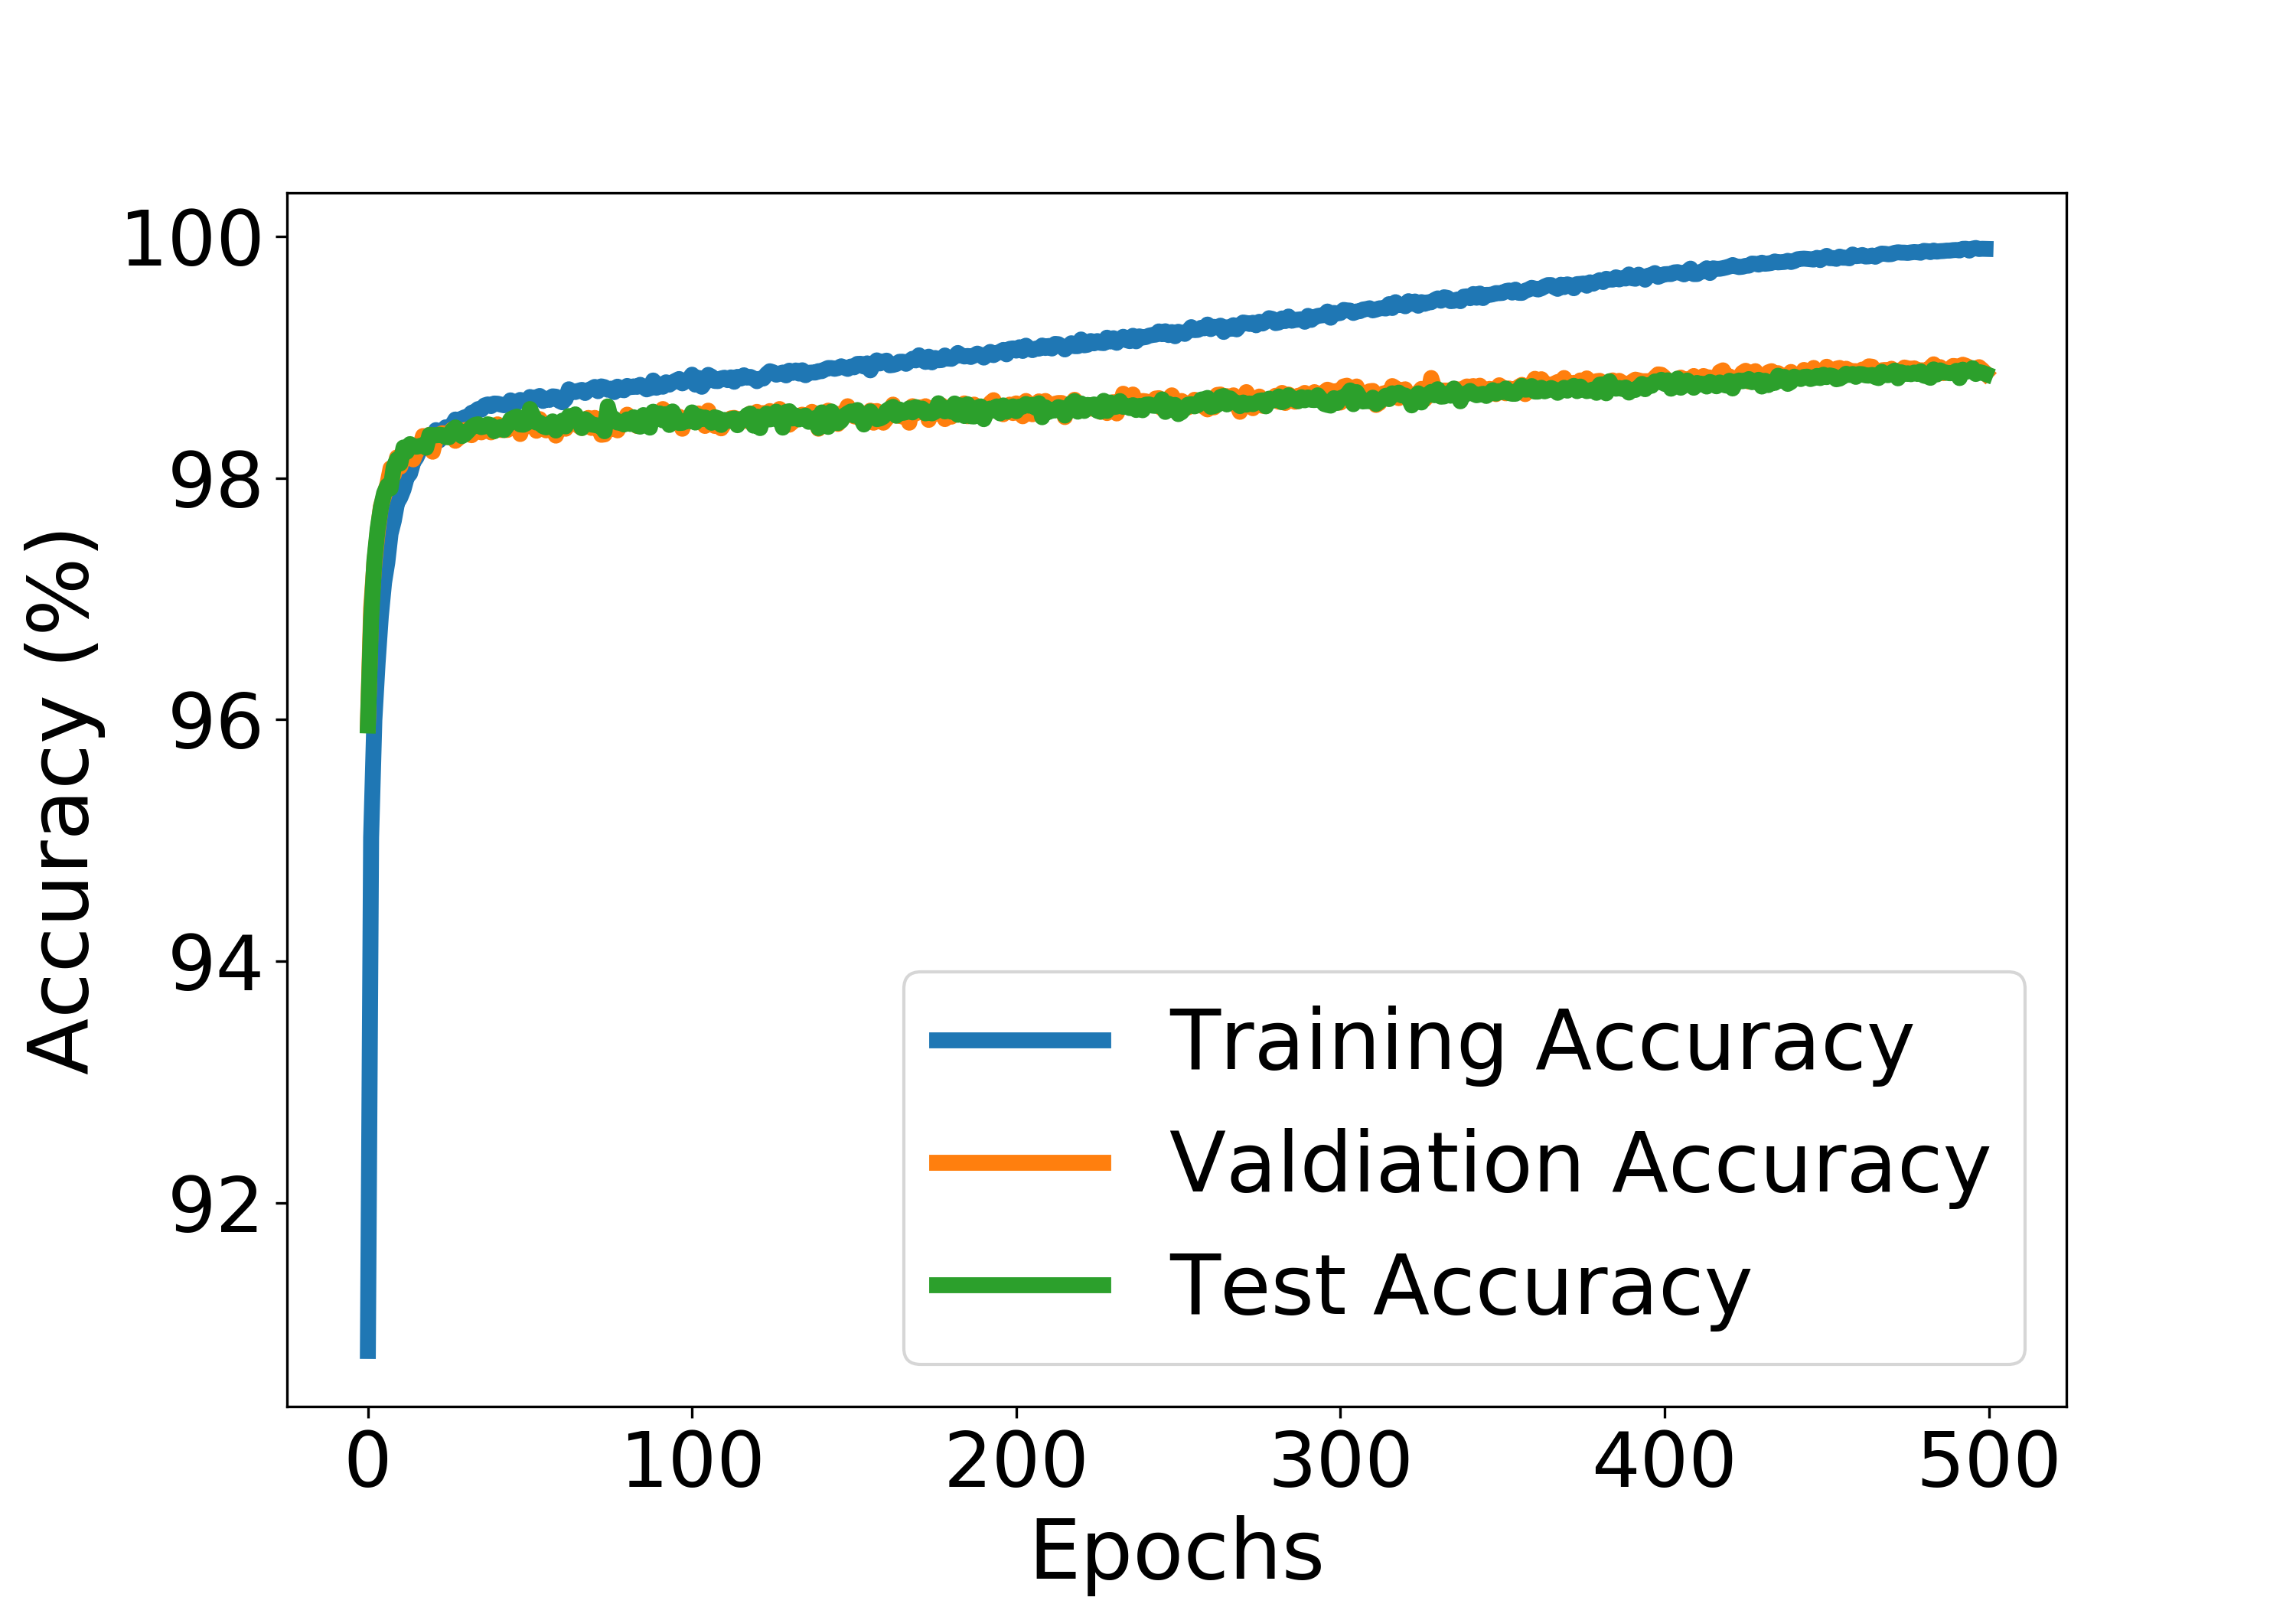
\includegraphics[width=1.2\textwidth]{../openreview/figs/MNIST.png}
         \caption{MNIST}
     \end{subfigure}
     \hfill
     \begin{subfigure}[b]{0.3\textwidth}
         \centering
         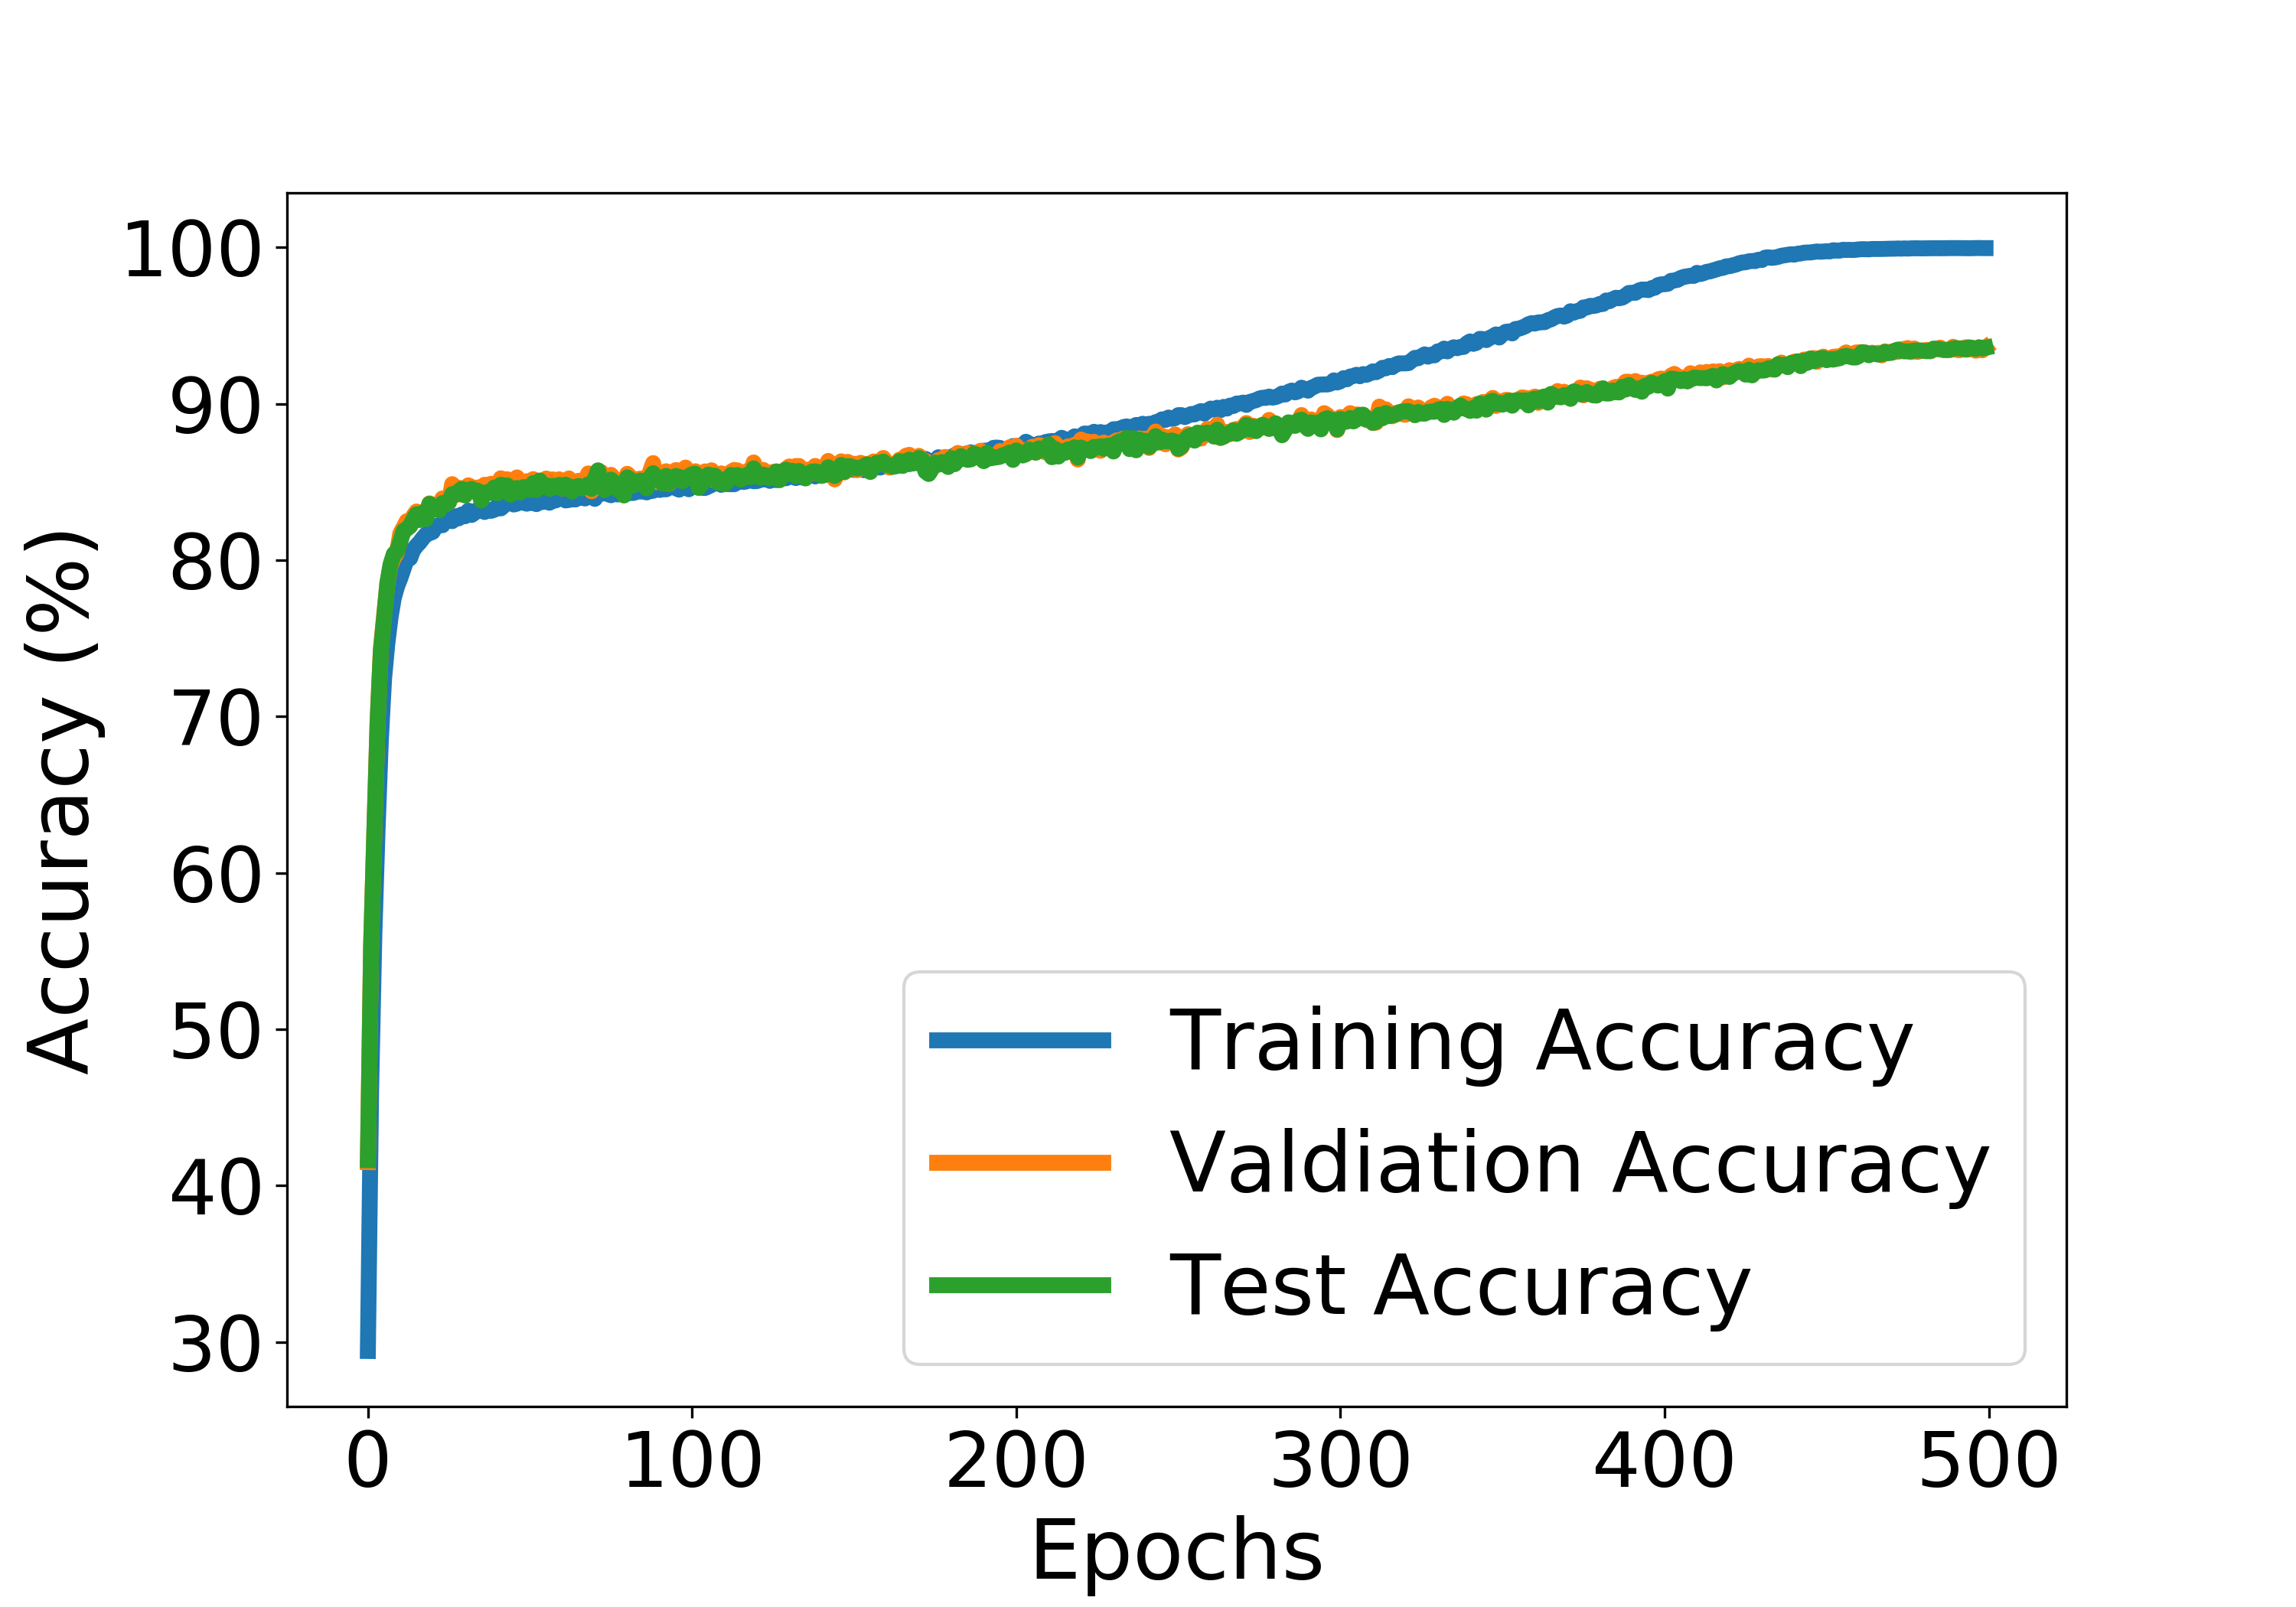
\includegraphics[width=1.2\textwidth]{../openreview/figs/CIFAR10.png}
         \caption{CIFAR10}
     \end{subfigure}
     \hfill
     \begin{subfigure}[b]{0.3\textwidth}
         \centering
         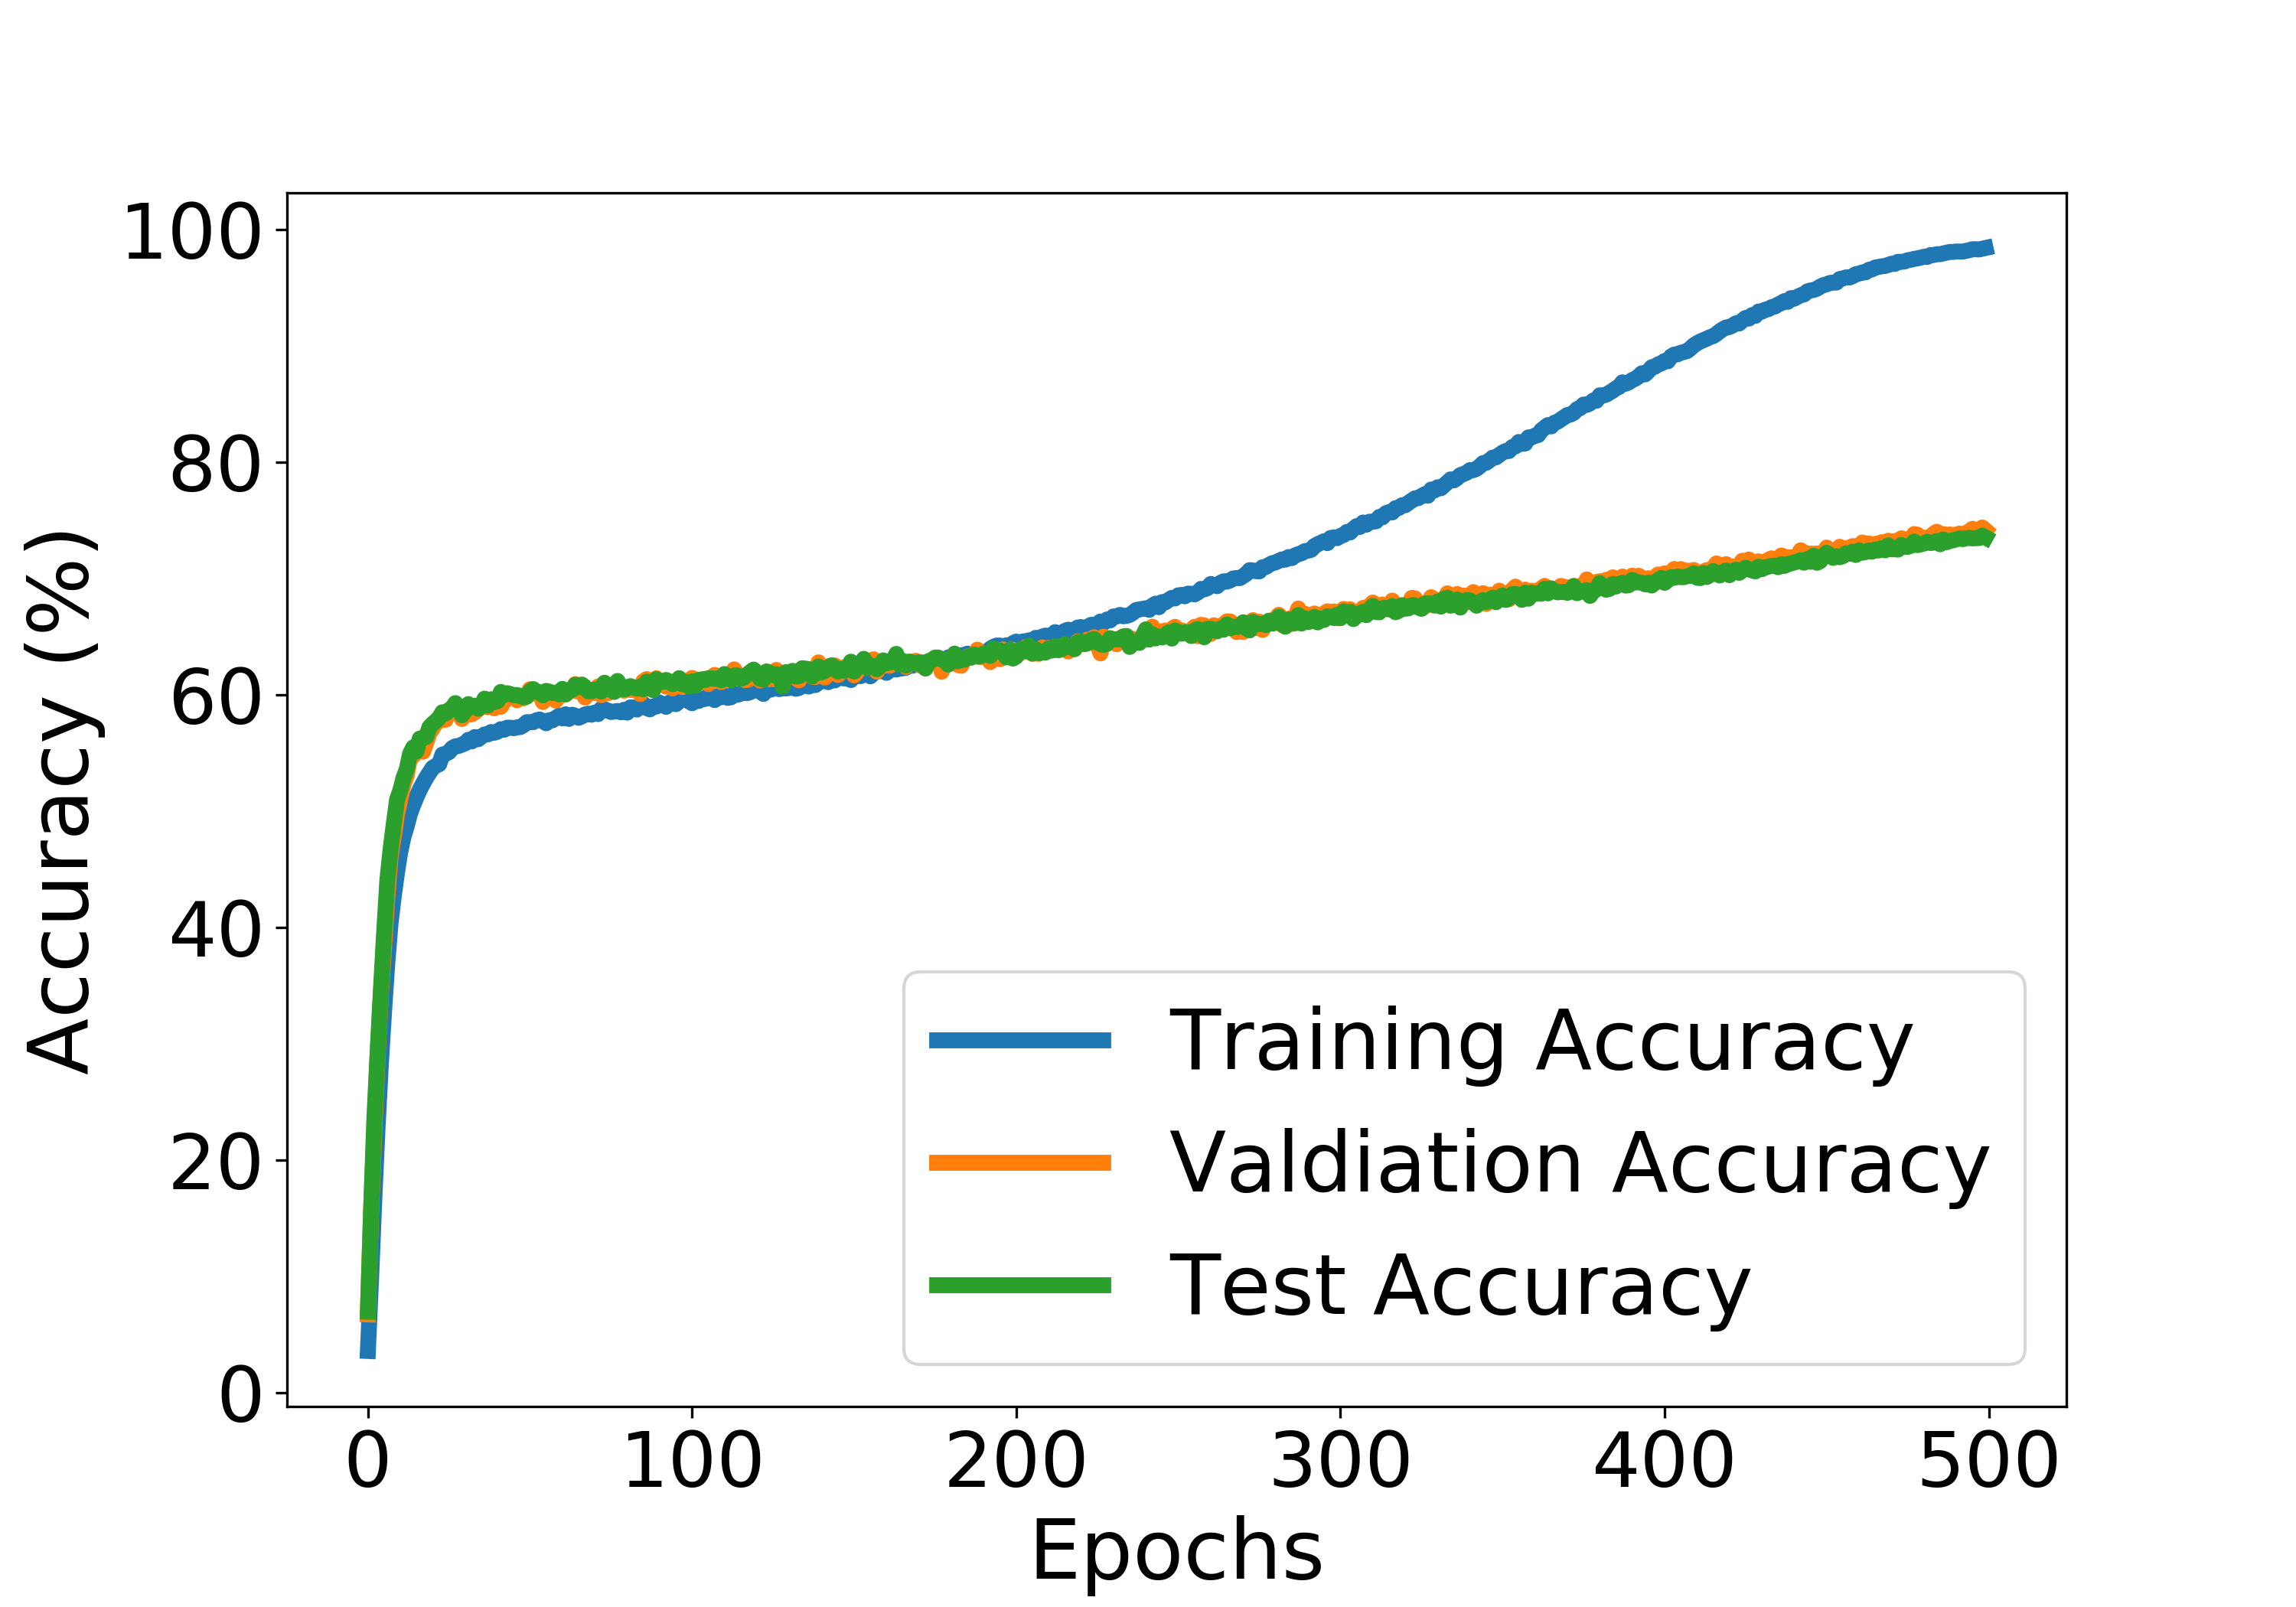
\includegraphics[width=1.2\textwidth]{../openreview/figs/CIFAR100.png}
         \caption{CIFAR100}
     \end{subfigure}
        \caption{Training/Validation/Test accuracy using BayesBiNN optimizer}
\end{figure}

\begin{table}[h]
\begin{center}
\small
\begin{tabular}{ | c | c | c | c | c | }
\hline
 Datasets & Optimizer & Training Accuracy & Validation Accuracy & Test Accuracy \\ \hline
  \multirow{5}{4em}{MNIST} 
   & BayesBiNN(ours) & $99.90 \pm 0.01\%$ & $99.89 \pm 0.07\%$ & $98.87 \pm 0.06\%$  \\
   & BayesBiNN(orig.) & $99.85 \pm 0.05\%$ & $99.02 \pm 0.13\%$ & $98.86 \pm 0.05\%$  \\
   & STE & $99.90 \pm 0.01\%$ & $98.86 \pm 0.09\%$ & $98.89 \pm 0.05\%$  \\
   & PMF & - & $98.73\%$ & -  \\
   & Adam (Full Precision) & $99.98 \pm 0.01\%$ & $99.02 \pm 0.04\%$ & $99.02 \pm 0.01\%$  \\ 
\hline

  \multirow{5}{4em}{CIFAR10}
   & BayesBiNN(ours) & $99.96 \pm 0.01\%$ & $93.59 \pm 0.45\%$ & $93.54 \pm 0.26\%$  \\
   & BayesBiNN(orig.) & $99.96 \pm 0.01\%$ & $94.23 \pm 0.41\%$ & $93.72 \pm 0.16\%$  \\
   & STE & $99.99 \pm 0.01\%$ & $93.77 \pm 0.06\%$ & $93.54 \pm 0.08\%$  \\
   & PMF & - & $91.98\%$ & -  \\
   & Adam (Full Precision) & $99.99 \pm 0.01\%$ & $94.27 \pm 0.15\%$ & $94.38 \pm 0.16\%$  \\ 
\hline
   
   
  \multirow{5}{4em}{CIFAR100} 
   & BayesBiNN(ours) & $98.35 \pm 0.1\%$ & $74.13 \pm 0.78\%$ & $73.56 \pm 0.06 \%$ \\
   & BayesBiNN(orig.) & $98.02 \pm 0.18\%$ & $74.76 \pm 0.41\%$ & $73.68 \pm 0.31\%$  \\
   & STE & $99.22 \pm 0.03\%$ & $72.74 \pm 0.06\%$ & $73.25 \pm 0.26\%$  \\
   & PMF & - & $70.82\%$ & -  \\
   & Adam (Full Precision) & $99.89 \pm 0.02\%$ & $75.04 \pm 0.71\%$ & $74.80 \pm 0.39\%$  \\ \hline
\end{tabular}
\caption{Results of different optimizers trained on MNIST, CIFAR10, and CIFAR100.}
\label{tab:result_1}

\end{center}
\end{table}

\subsection{Comparison with LR-Net}
Authors compared their BayesBiNN approach to the LR-Net method presented in \citet{r8}. We tried to reproduce the result for the same setting. In this comparison, the data pre-processing and augmentation methods remain the same as mentioned in section 4.2, but we do not split the data in training and validation sets in this case. We denote the test accuracies after 190 epochs in the case of MNIST and 290 epochs in the case of CIFAR-10, as done in the original paper to maintain uniformity. Note that, our accuracy is matching with that of the original authors in the case of MNIST but not in the case of CIFAR-10. We suspect that this is due to some difference in Batch-Norm layers used.

\begin{table}[h]
\begin{center}
\renewcommand{\arraystretch}{1.1}
\begin{tabular}{ | c | c | c |}
\hline
 Optimizer & MNIST &  CIFAR10 \\ \hline
%   \multirow{2}{5em}{MNIST} 
   BayesBiNN (ours) & \textbf{99.52\%} & $84.49\%$ \\ \hline
   BayesBiNN (orig.) & $99.50\%$ & $\textbf{93.97\%}$ \\ \hline
   LR-net \citet{r8} & $99.47\%$ & $93.18\%$ \\
\hline
\end{tabular}
\caption{Test accuracy of BayesBiNN and LRNet.}
\label{tab:LR_result_2}

\end{center}
\end{table}

\subsection{Continual Learning}
As mentioned in the original paper, we try to reproduce the author's claims about weight distribution across tasks in a simple continual learning domain tested on Permuted MNIST. Clearly, as we learn across the tasks, the curve becomes flat from the middle conveying that the weights become more deterministic. Our result matches with the claims in the original paper.
\begin{figure}[h]
     \centering
     \begin{subfigure}[b]{0.3\textwidth}
         \centering
         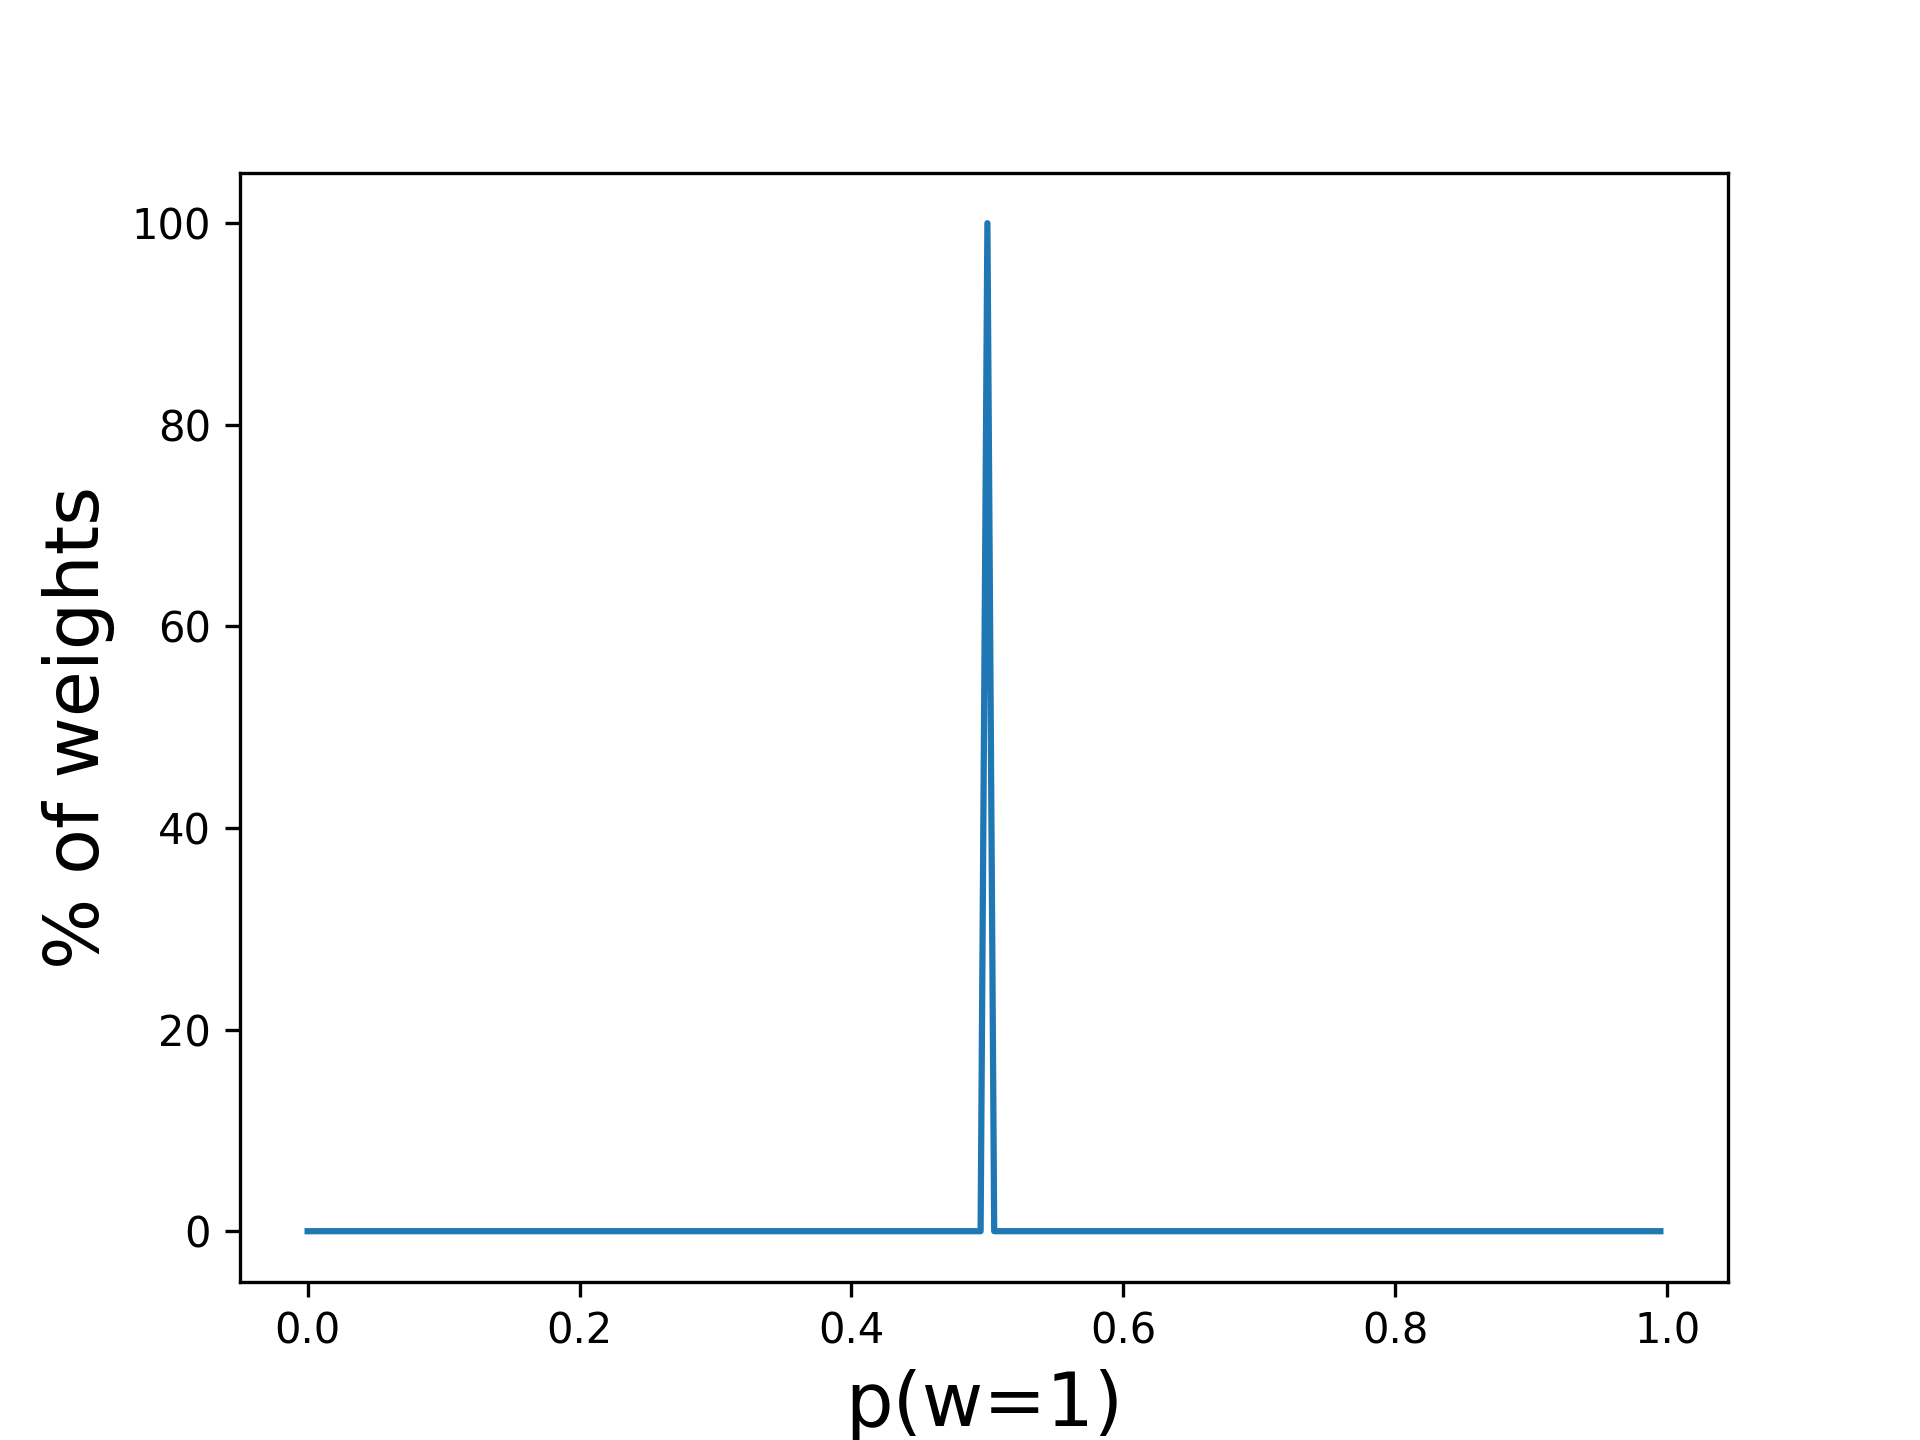
\includegraphics[width=1.1\textwidth]{../openreview/figs/after_task_0.png}
         \caption{Prior $\lambda$}
     \end{subfigure}
     \hfill
     \begin{subfigure}[b]{0.3\textwidth}
         \centering
         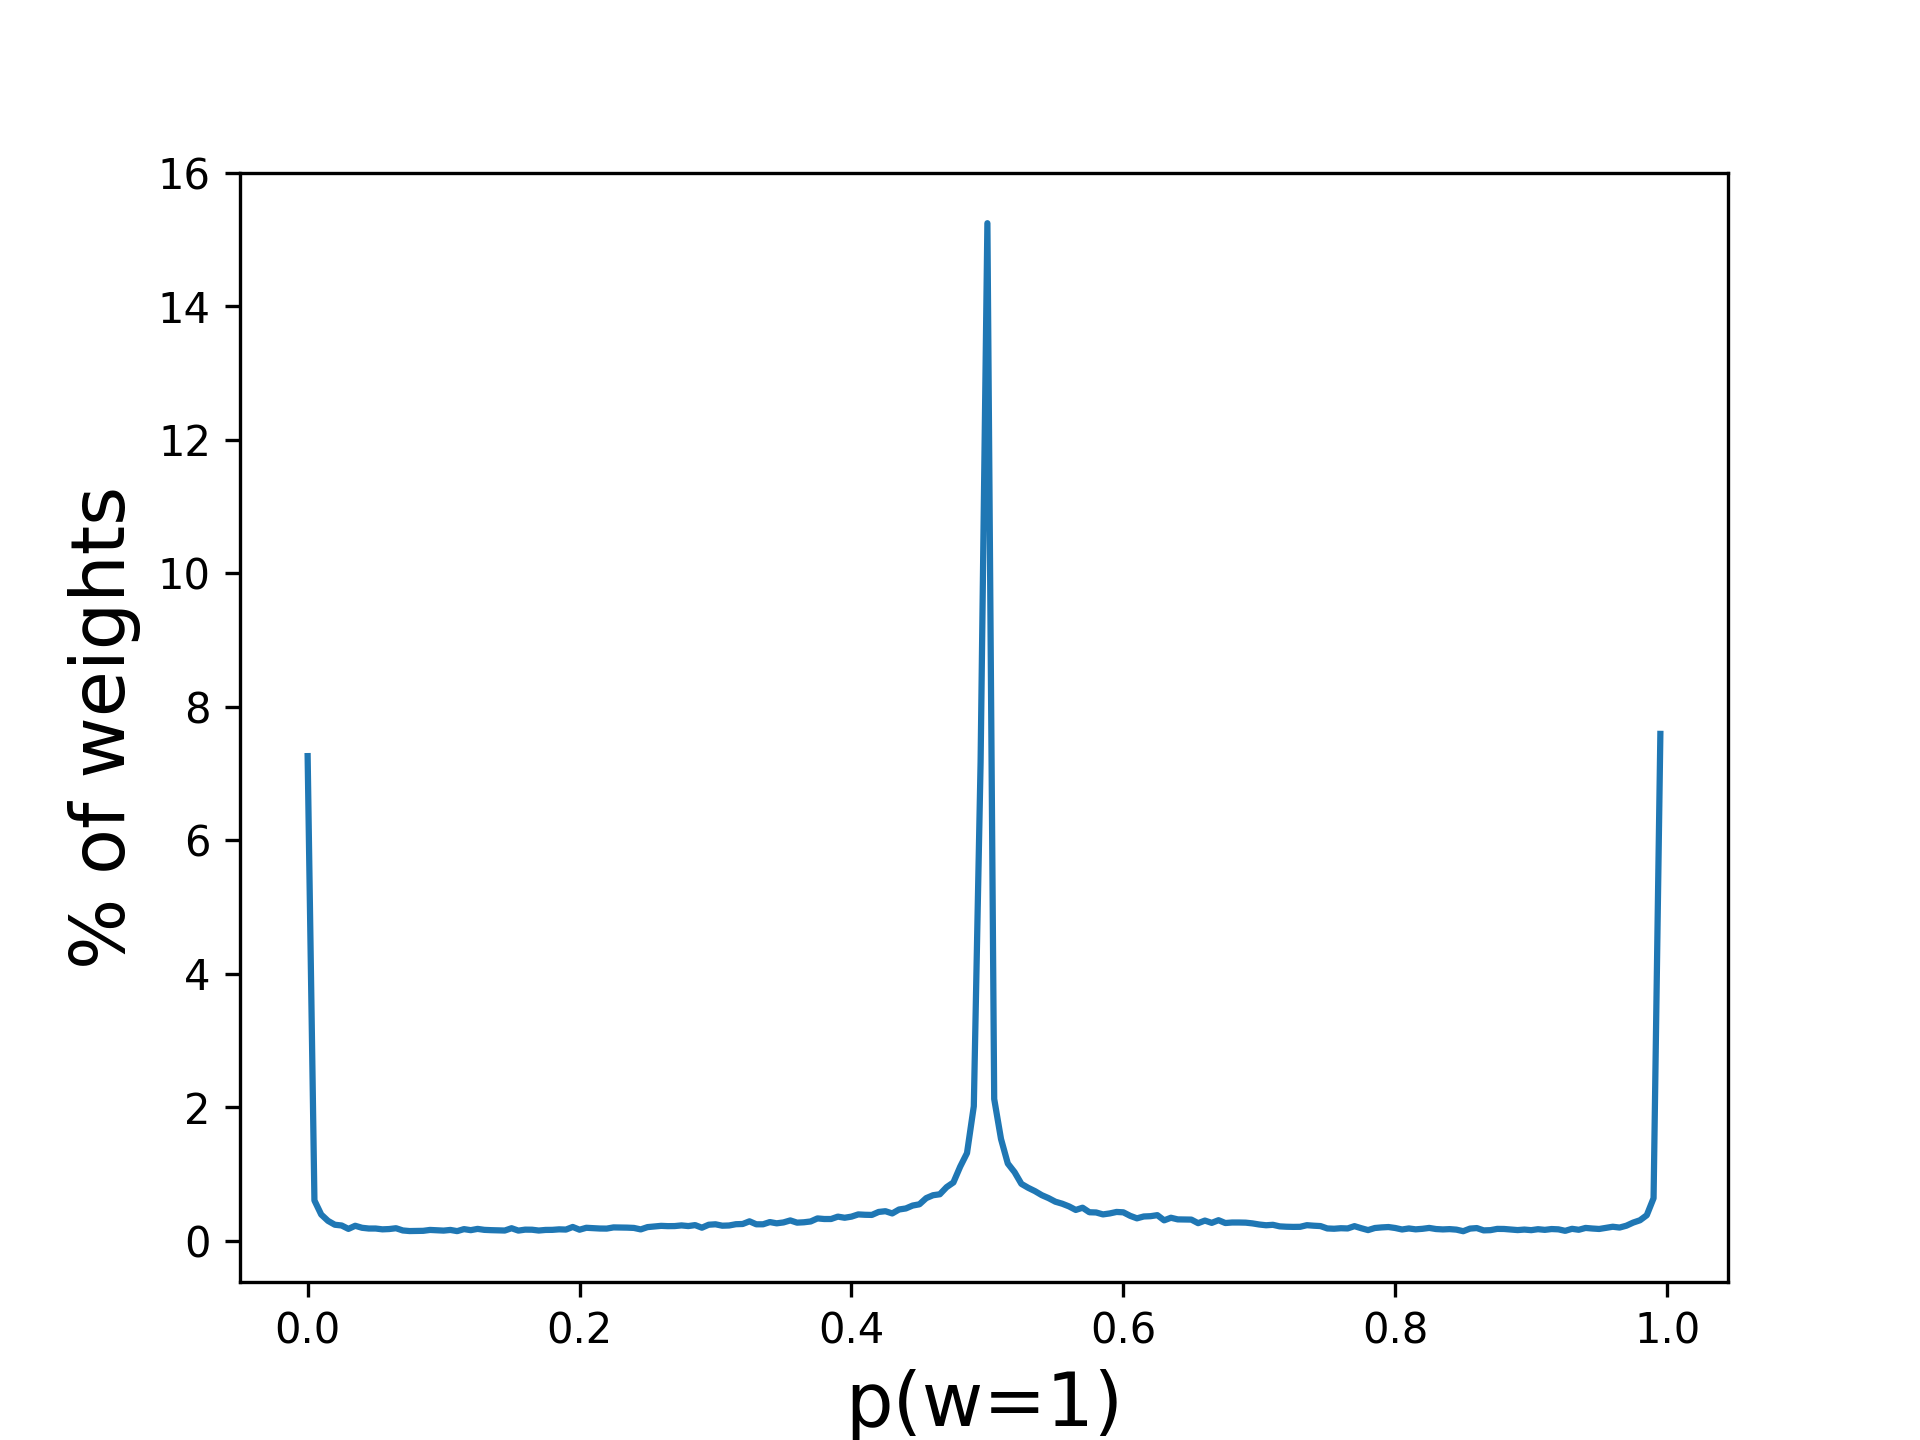
\includegraphics[width=1.1\textwidth]{../openreview/figs/after_task_1.png}
         \caption{$\lambda$ after task 1}
     \end{subfigure}
     \hfill
     \begin{subfigure}[b]{0.3\textwidth}
         \centering
         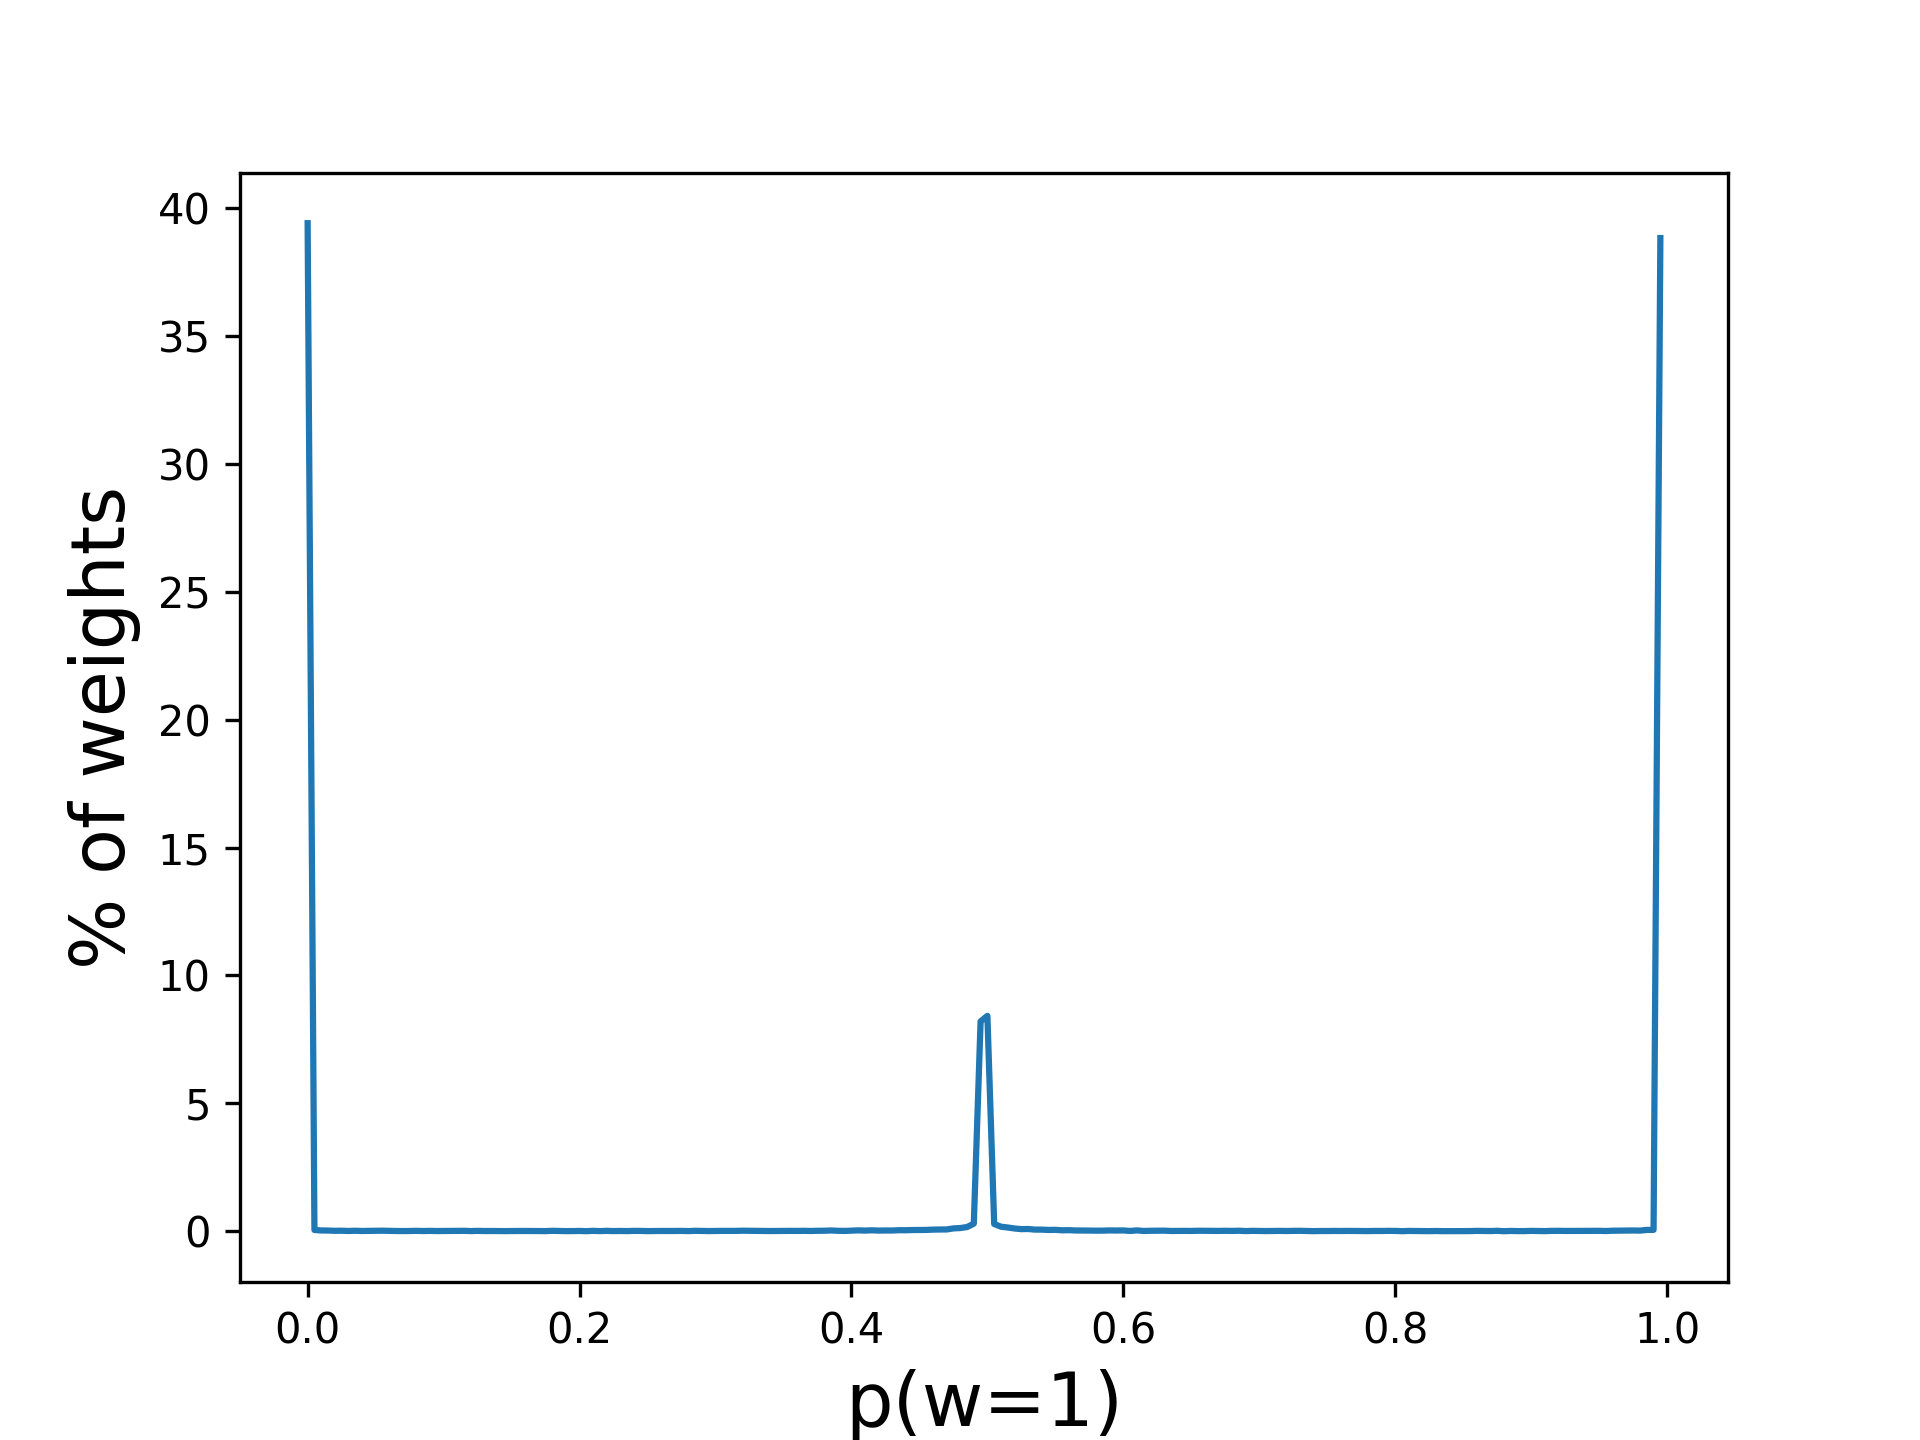
\includegraphics[width=1.1\textwidth]{../openreview/figs/after_task_2.png}
         \caption{$\lambda$ after task 2}
     \end{subfigure}
        \caption{Distribution of $p(w=1)$ across consecutive learning tasks}
\end{figure}

\subsection{Visualization using Synthetic Dataset}

In the original paper, the authors present visualizations on binary classification (Two moons dataset \citet{r10}) and toy regression (Snelson dataset \citet{r9}) using STE and BayesBiNN optimizer. For the classification task, the authors claimed that STE is a more deterministic classifier compared to BayesBiNN. We reproduced this experiment and the results depicted in Figure \autoref{fig3} seem to be consistent with the author's claim. For the regression task, we conclude that the author's claim about BayesBiNN (mean) giving a smoother curve compared to STE is true, which can also be seen in Figure \autoref{fig4}. 


\begin{figure}[h]
     \centering
         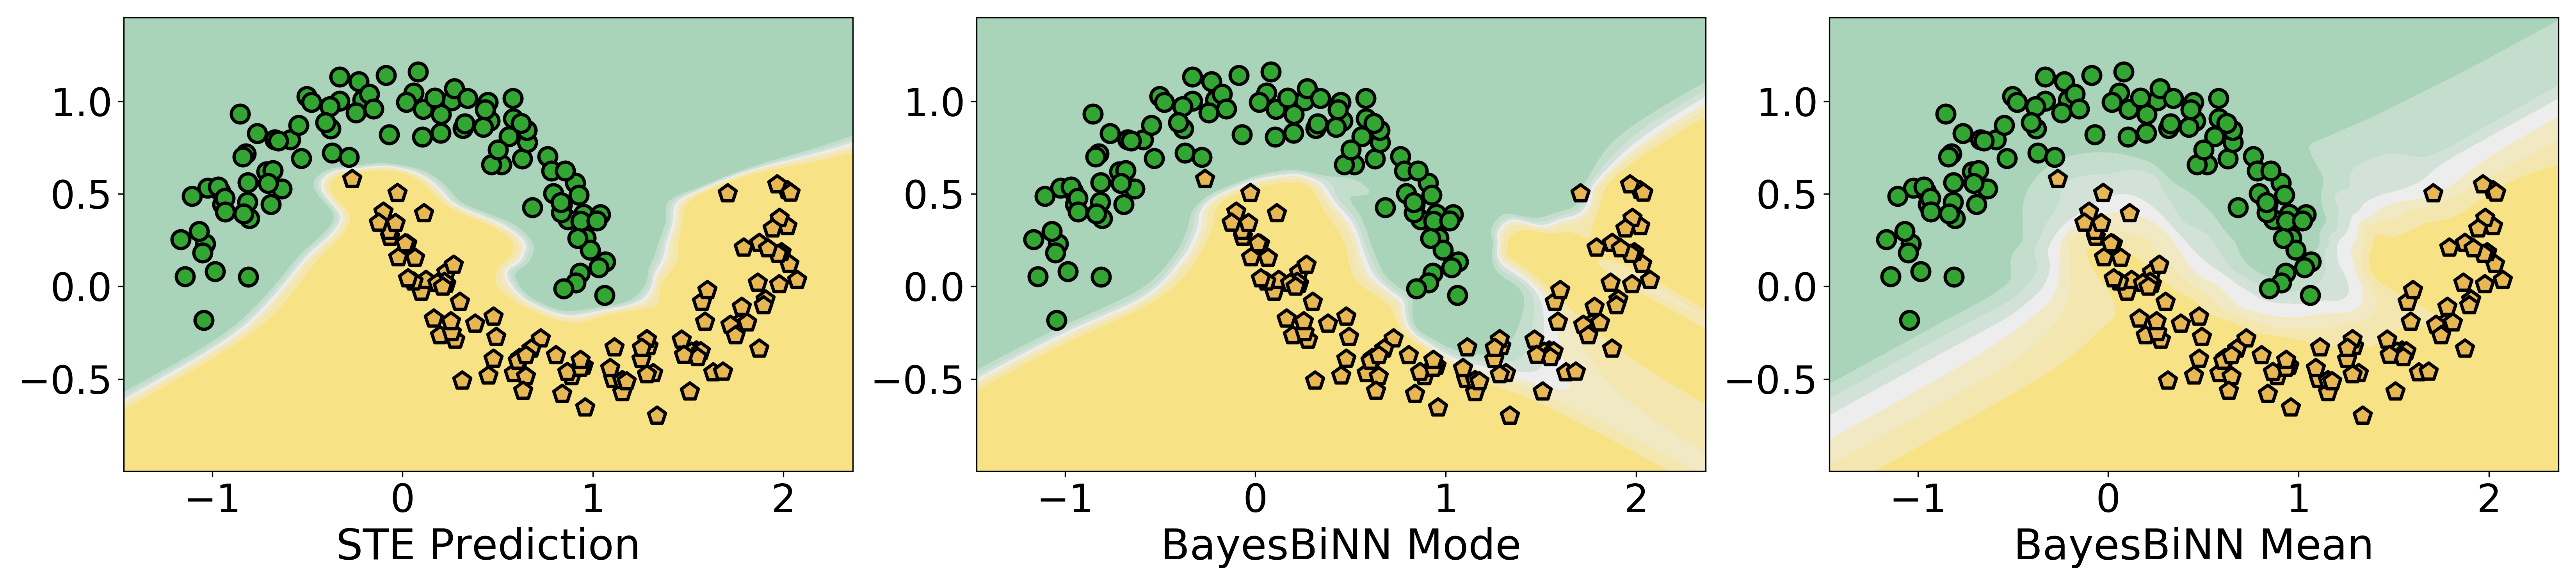
\includegraphics[width=1\textwidth]{../openreview/figs/TwoMoon.png}
         \caption{Classification on Two Moons dataset using STE and BayesBiNN optimizer.}
         \label{fig3}
\end{figure}

\begin{figure}[h]
     \centering
         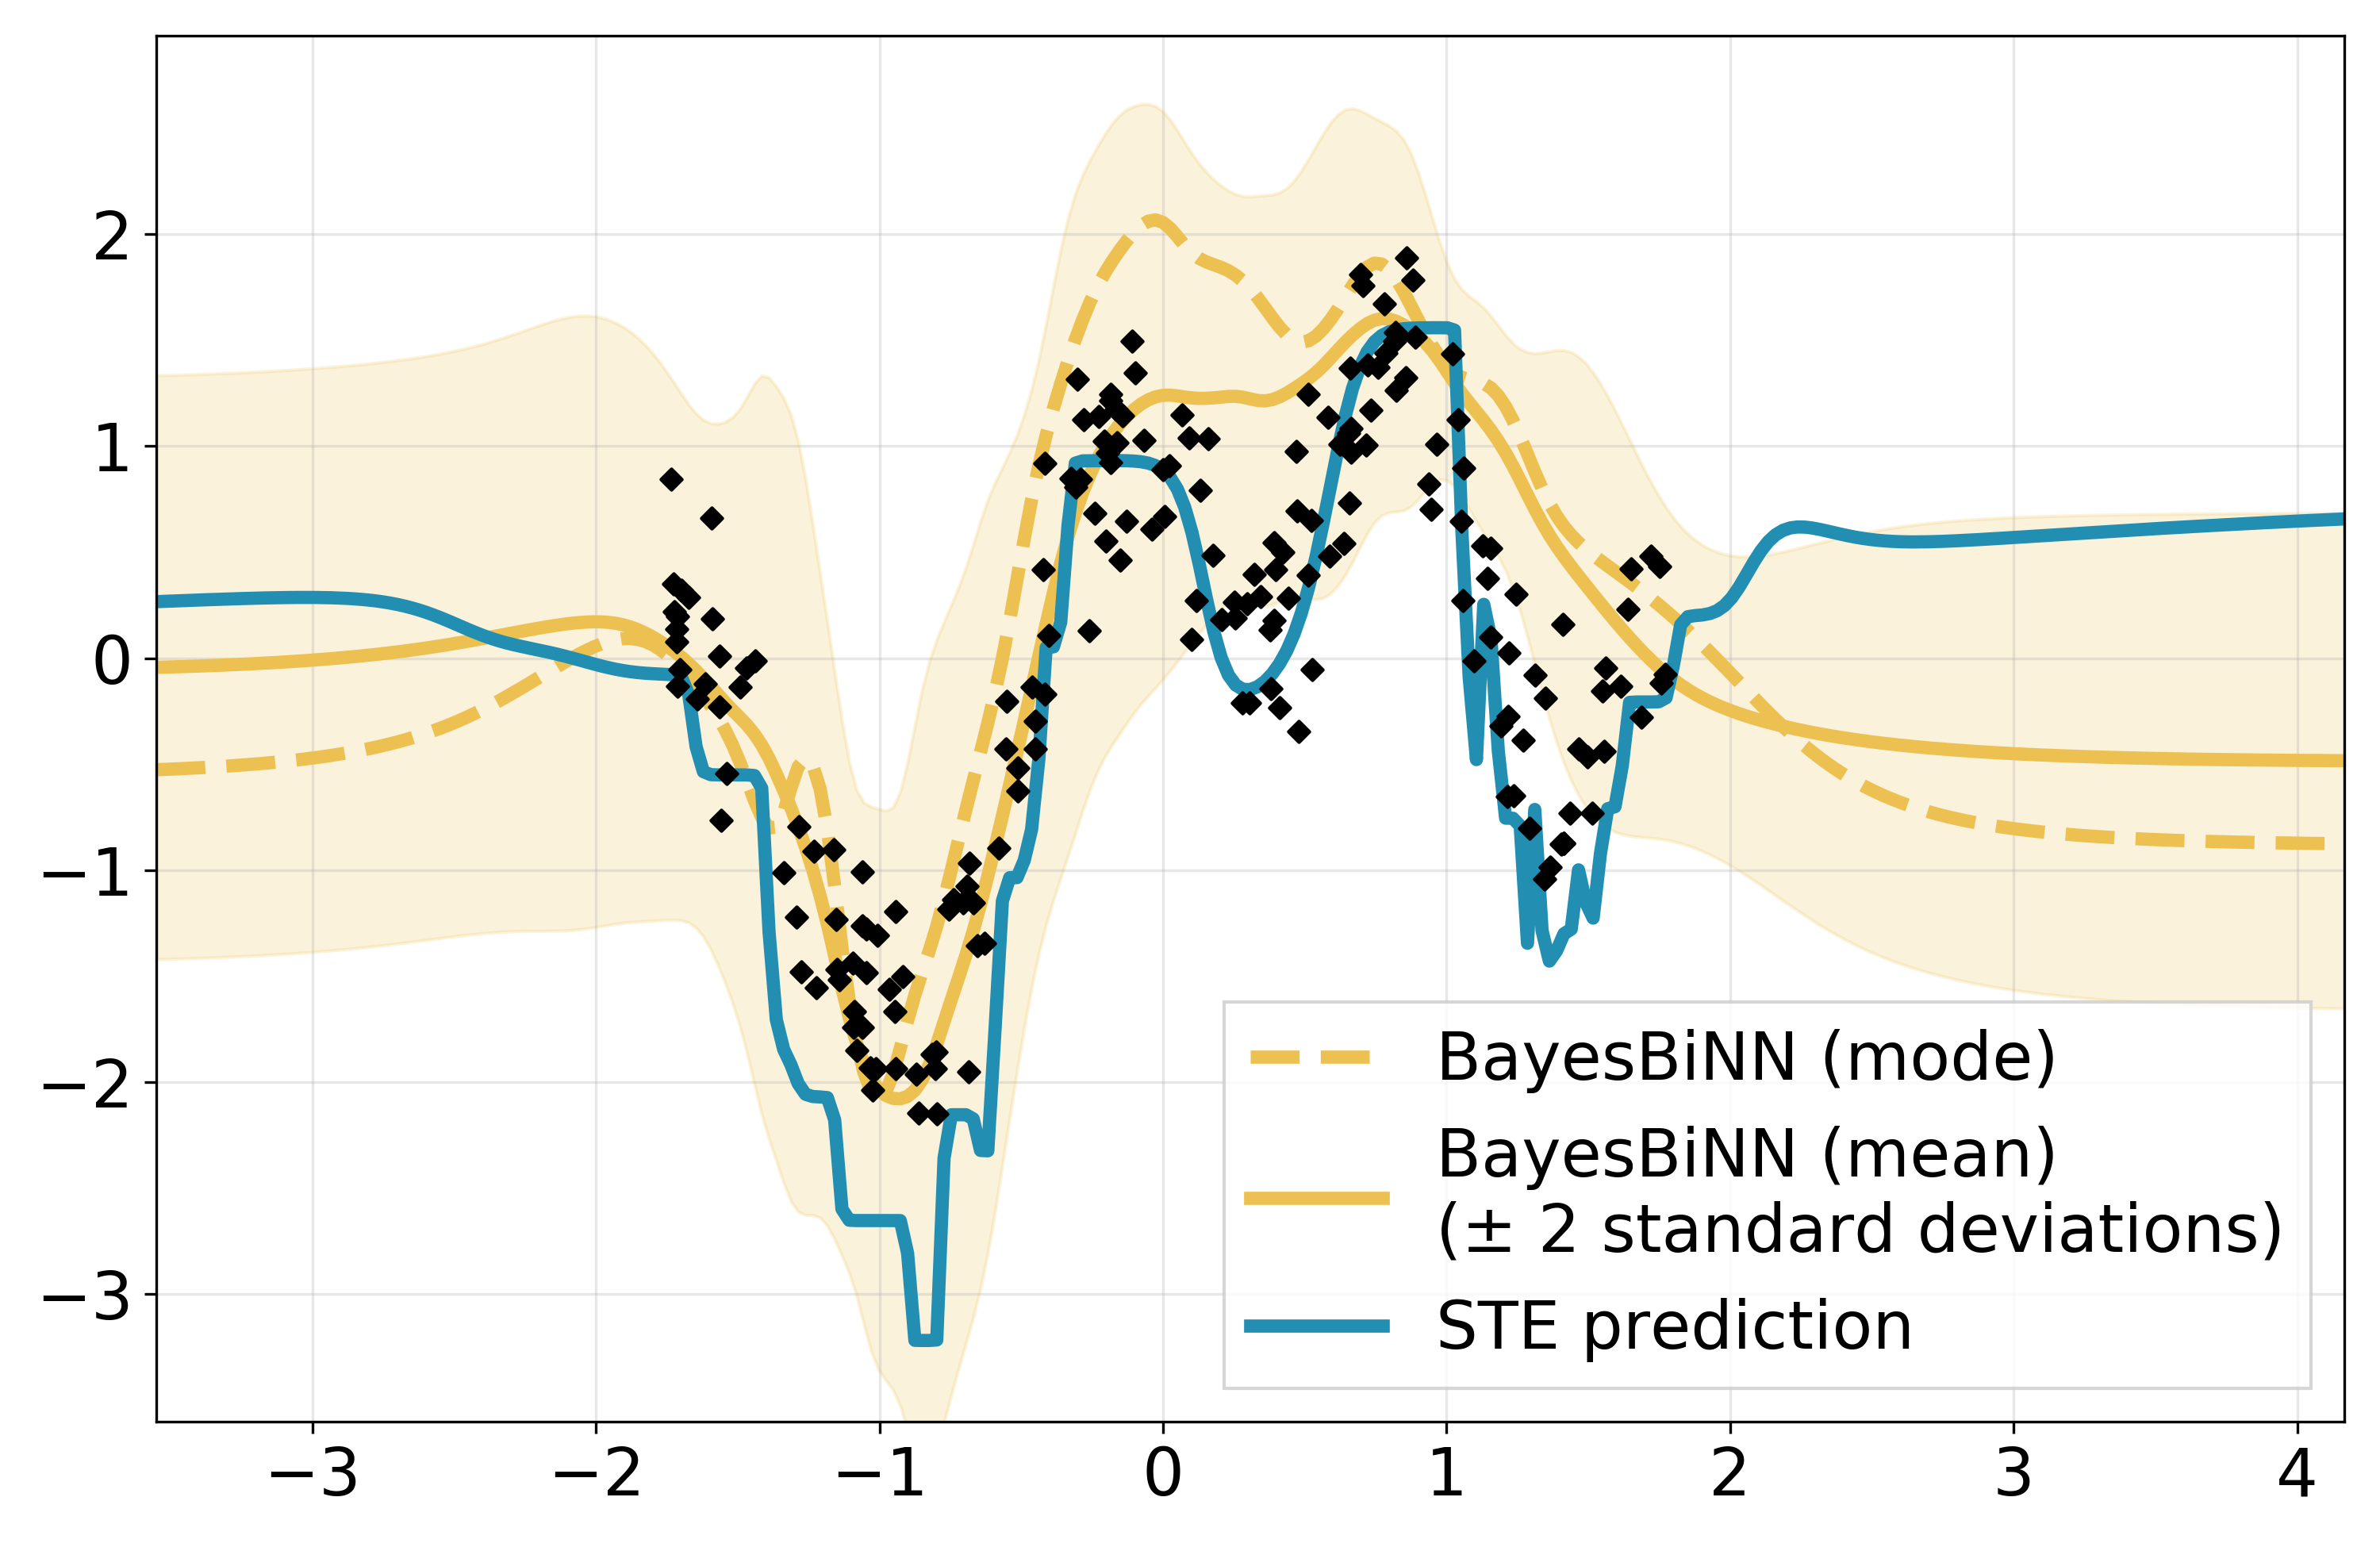
\includegraphics[width=0.6\textwidth]{../openreview/figs/Snelson.png}
         \caption{Regression on Snelson dataset using STE and BayesBiNN optimizer.}
         \label{fig4}
\end{figure}


\begin{table}[h]
\begin{center}
\setlength{\tabcolsep}{12pt}
\renewcommand{\arraystretch}{1.3}
\begin{tabular}{ | c | c | c | c | c | c | c | }
\hline
 \textbf{Temperature} & 10 & 1 & 0.1 & $10^{-2}$ & $10^{-3}$ & $10^{-4}$ \\\hline
 MSE Loss & 1.313 & 0.208 & 2.151 & 0.443 & 0.231 & 0.199\\ \hline
 \textbf{Temperature} & $10^{-5}$ & $10^{-6}$ & $10^{-7}$ & $10^{-8}$ & $10^{-9}$ & $10^{-10}$\\  \hline
 MSE Loss & 0.156 & 0.127 & 0.173 & 0.122 & 0.195 & 0.173\\ 
\hline
\end{tabular}
\caption{Mean square error loss of Snelson dataset for different temperatures.}
\label{tab:Ablation_result_4}

\end{center}
\end{table}

\subsection{Extended Results (Semantic Segmentation)}
We tried to validate the performance of the BayesBiNN optimizer on more complex tasks like semantic segmentation. Unfortunately, the results with BayesBiNN were quite underwhelming as compared to STE and its full-precision counterpart. We tried various parameters to improve its performance but none seemed to work. We had a brief discussion with the authors regarding this issue and the authors suggested that Bayesian models are intrinsically very difficult to train. For the results shown in Table \autoref{tab:table5} and Figure \autoref{fig5}, we have used the hyperparameters denoted in Table \autoref{tab:table1}.

\begin{table}[h]
\begin{center}
\renewcommand{\arraystretch}{1.1}
\begin{tabular}{ | c | c | c | c |}
\hline
  & BayesBiNN & STE &  Adam (Full Precision) \\ \hline
    Validation Score & 0.4102 & 0.3108 & 0.2943 \\ \hline
\end{tabular}
\caption{(1 - IoU) score for validation set}
\label{tab:table5}
\end{center}
\end{table}

\begin{figure}[h]
     \centering
     \begin{subfigure}[b]{0.3\textwidth}
         \centering
         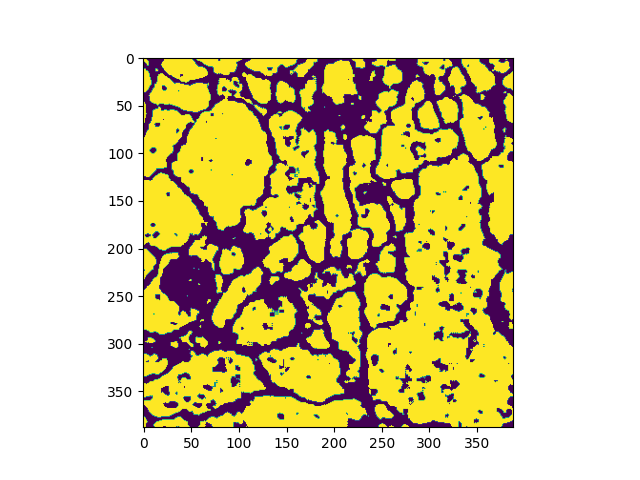
\includegraphics[width=1.3\textwidth]{../openreview/figs/output_bayesbinn.png}
         \caption{BayesBiNN}
     \end{subfigure}
     \hfill
     \begin{subfigure}[b]{0.3\textwidth}
         \centering
         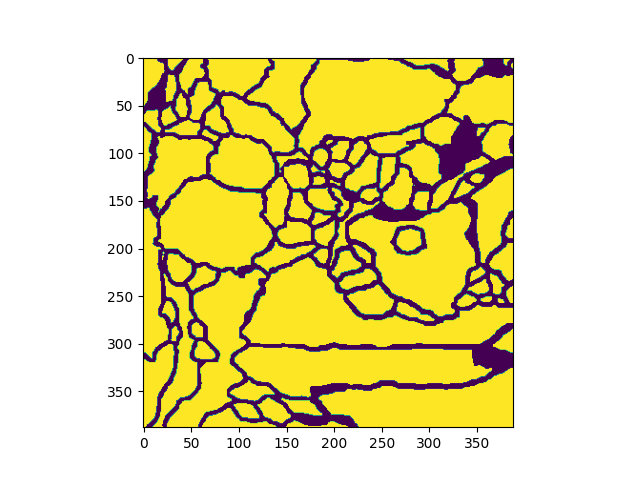
\includegraphics[width=1.3\textwidth]{../openreview/figs/output_ste.png}
         \caption{STE}
     \end{subfigure}
     \hfill
     \begin{subfigure}[b]{0.3\textwidth}
         \centering
         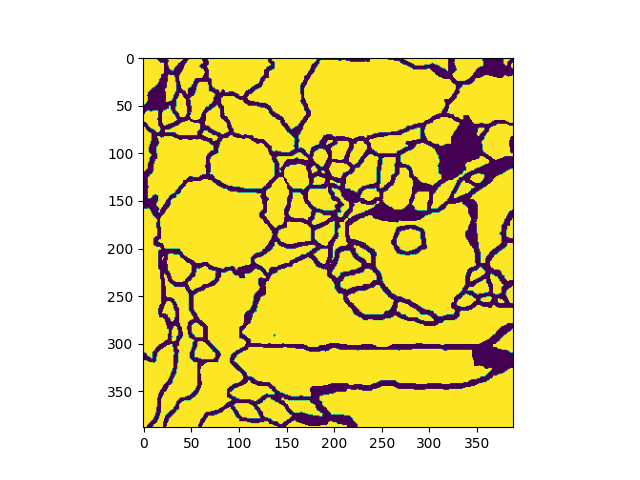
\includegraphics[width=1.3\textwidth]{../openreview/figs/output_normal.png}
         \caption{Adam}
     \end{subfigure}
        \caption{Some samples of segmented image outputs}
        \label{fig5}
\end{figure}

\subsection{Results beyond original paper}
%Often papers don't include enough information to fully specify their experiments, so some additional experimentation may be necessary. For example, it might be the case that batch size was not specified, and so different batch sizes need to be evaluated to reproduce the original results. Include the results of any additional experiments here. Note: this won't be necessary for all reproductions.
This section includes the results for SMAE, our extension of the MAE which combines pixel-wise loss and perceptual loss. Results for using only perceptual loss (SMAE with $\alpha=1$) are deferred to Appendix E.

\subsubsection{SMAE}
The results from our proposed SMAE are presented in Table \ref{tab:results}. The SMAE performed similarly to the MAE when fine-tuned on TIN. When transferred to CUB, our extension performs well, improving the performance of the MAE by a large margin (+5 pp). The respectable performance of the SMAE provides further evidence in support of claim \ref{generalization}. Regarding the masking method for SMAE, the choice between random masking and block masking did not have a significant impact on performance when fine-tuning on TIN. When transferred to CUB, SMAE displayed significantly greater performance with block masking than random masking (+6.0 pp) in terms of validation set accuracy.
% \setlength{\tabcolsep}{6pt}
% \begin{table*}[!ht]
% \begin{center}
% \begin{tabular}{@{}lll@{}}
% \toprule
% \multicolumn{3}{c}{SMAE} \\
%        & TIN    & CUB    \\
% Random & 0.00\% & 0.00\% \\
% Block  & 0.00\% & 0.00\%
% \end{tabular}
%         % \vspace{}
%         \caption{Ablation of the SMAE masking strategy.}
%         \label{tab:smae_masking}
%     \end{center}
% \end{table*}

\begin{center}\vspace{-.2em}
\tablestyle{6pt}{1.2}
\begin{tabular}{ c c c c }
\multicolumn{2}{c}{} & TIN & CUB \\
\shline
\multirow{2}{*}{Masking} & Random & \textbf{54.40} & 41.50 \\
& Block & 53.90 & \textbf{47.50} 
\end{tabular}\vspace{-.2em}
\end{center}

\section{Discussion}

%\textit{Give your judgement on if your experimental results support the claims of the paper. Discuss the strengths and weaknesses of your approach - perhaps you didn't have time to run all the experiments, or perhaps you did additional experiments that further strengthened the claims in the paper.}\\

Our experimental results support the main claims of \cite{mae} that we set out to reproduce, i.e. claim \ref{nontrivial} and \ref{generalization}. Due to our significant computational constraints, we have not attempted to reproduce experiments supporting claim \ref{scalability}. We conclude that the MAE framework is reproducible in general, and that it also performs well with smaller datasets and backbones. A weakness of our reproducibility approach is the comparison between MAE and DINO. Due to our limited resources and the high computational demand of DINO, we could not perform a proper grid search for it. Provided this, our comparison between MAE and DINO is not entirely fair.
\\\\
We have also presented the SMAE, an extension to the MAE that incorporates recent ideas about using perceptual loss to improve the usefulness of embeddings. Our results suggest that the SMAE learns semantically meaningful representations that are more useful than those of the MAE when transferring to another dataset. It should be noted that our results on transfer learning only concern one dataset. Extending the experiments to more datasets would be necessary to corroborate our findings regarding the improved performance of SMAE. Future research could further investigate loss weighting and choice of perceptual network for the SMAE; something that was out-of-scope for this study.
\\\\
The authors of BootMAE \cite{bootmae} observed that training with perceptual loss benefits from masking out larger connected blocks. Our findings for transferring SMAE to CUB align with this, as we see a big performance increase when going from random masking to block masking. In contrast, fine-tuning SMAE on TIN did not express any meaningful performance difference with respect to the masking method. This result suggests that the choice of masking method might be more important when transferring to a different data distribution.

\subsection{What was easy}
%\textit{Give your judgement of what was easy to reproduce. Perhaps the author's code is clearly written and easy to run, so it was easy to verify the majority of original claims. Or, the explanation in the paper was really easy to follow and put into code. }

%\textit{Be careful not to give sweeping generalizations. Something that is easy for you might be difficult to others. Put what was easy in context and explain why it was easy (e.g. code had extensive API documentation and a lot of examples that matched experiments in papers).}\\

Given prior experience with a deep learning framework, re-implementing the paper was relatively straight-forward, with exception for the random shuffling and un-shuffling (see Section \ref{sec:difficult}). The paper provided sufficient details on the MAE method, including training configurations and implementational details.

\subsection{What was difficult}
\label{sec:difficult}
%\textit{List part of the reproduction study that took more time than you anticipated or you felt were difficult. }

%\textit{Be careful to put your discussion in context. For example, don't say "the maths was difficult to follow", say "the math requires advanced knowledge of calculus to follow". }\\

It was not trivial to apply the approach in the paper on a different choice of dataset and backbone, as the paper's choices of hyperparameters turned out to require significant recalibration. Therefore, we had to spend quite some time tuning hyperparameters. We temporarily struggled with the details of implementing random shuffling and un-shuffling of patches correctly \textit{and} efficiently. Our final implementation for the shuffling and un-shuffling operations used the scatter and gather functions in PyTorch, which are fairly involved operations. 
% \\\\
% Another aspect that we found quite uneasy to reproduce was the scalability experiments conducted in \cite{mae}, justifying claim \ref{scalability}. In particular, we starting pre-training 

\subsection{Communication with original authors}
%\textit{Document the extent of (or lack of) communication with the original authors. To make sure the reproducibility report is a fair assessment of the original research we recommend getting in touch with the original authors. You can ask authors specific questions, or if you don't have any questions you can send them the full report to get their feedback before it gets published. }\\

We have not had contact with the original authors.
